%\documentclass[pdflatex,11pt]{aghdpl}
\documentclass{aghdpl}               % przy kompilacji programem latex
% \documentclass[pdflatex,en]{aghdpl}  % praca w j�zyku angielskim
\usepackage[polish]{babel}
\usepackage[cp1250]{inputenc}

% dodatkowe pakiety
\usepackage{hyperref}
\usepackage{enumerate}
\usepackage{listings}
\usepackage{algorithm}
\usepackage{algpseudocode}
\lstloadlanguages{TeX}


%---------------------------------------------------------------------------

\author{Pawe� K�eczek}
\shortauthor{P. K�eczek}

\titlePL{Symulacja ruchu ludzi w galerii handlowej}
\titleEN{A simulation of pedestrian behavior in a shopping mall}

\shorttitlePL{Symulacja ruchu ludzi w galerii handlowej}
\shorttitleEN{A simulation of pedestrian behavior in a shopping mall}

\thesistypePL{Praca in�ynierska}
\thesistypeEN{Bachelor of Science Thesis}

\supervisorPL{dr in�. Jaros�aw W�s}
\supervisorEN{Jaros�aw W�s Ph.D}

\date{2013}

\departmentPL{Katedra Informatyki Stosowanej}
\departmentEN{Department of Applied Computer Science}

\facultyPL{Wydzia� Elektrotechniki, Automatyki, Informatyki i In�ynierii Biomedycznej}
\facultyEN{Faculty of Electrical Engineering, Automatics, Computer Science and Biomedical Engineering}

\acknowledgements{} % podzi�kowania


\setlength{\cftsecnumwidth}{10mm}

%---------------------------------------------------------------------------

\begin{document}

%\titlepages

%\tableofcontents
%\clearpage

%\chapter{Wprowadzenie}
\label{cha:wprowadzenie} 
 
 Zagadnienie modelowania ruchu i zachowania pieszych jest od d�ugiego czasu postrzegane jako istotne z punktu widzenia sektora us�ugowego i handlowego. Przekonanie to znajduje potwierdzenie w badaniach przytoczonych cho�by  przez Aloysa Borgersa i Harry'ego Timmermansa \cite{BoTi86-1}, kt�re wykaza�y wysok� zale�no�� rentowno�ci sklep�w od sposobu poruszania si� potencjalnych klient�w. Problem ten jest do�� z�o�ony i dodatkowo mo�e by� rozwa�any na r�nych poziomach abstrakcji, w zale�no�ci od przeznaczenia modelu.
 
%---------------------------------------------------------------------------

\section{Cele pracy}
\label{sec:celePracy}

Celem niniejszego projektu jest opracowanie modelu ruchu ludzi w centrum handlowym oraz stworzenie na jego podstawie symulacji komputerowej, kt�ra pozwoli oceni� jako�� modelu.

%---------------------------------------------------------------------------

\section{Zawarto�� pracy}
\label{sec:zawartoscPracy}

G��wna cz�� pracy sk�ada si� z pi�ciu rozdzia��w. W rozdziale 2 dokonano przegl�du r�nych podej�� do zagadnienia modelowania przemieszczania si� pieszych. W rozdziale 3 przedstawiono stworzony na potrzeby projektu model centrum handlowego. W rozdziale 4 om�wiono algorytmy stosowane do modelowania ruchu pieszych. Rozdzia� 5 zawiera opisy szczeg��w implementacyjnych. Rozdzia� 6 prezentuje wyniki symulacji i ich analiz�.

%\chapter{Analiza obecnych rozwi�za�}
\label{cha:sota}

W rozdziale tym przedstawiono klasyfikacj� zachowania agent�w oraz dokonanu przegl�du niekt�rych ze stosowanych obecnie podej�� do modelowania ruchu pieszych. Poniewa� w niniejszej pracy zastosowane zosta�o podej�cie wieloagentowe, zostanie ono om�wione szczeg�owo w kolejnych rozdzia�ach.

%---------------------------------------------------------------------------

\section{Zachowanie agent�w}
\label{sec:behavior}

Norma \emph{ISO/TR 13387-1:1999 Fire safety engineering} \cite{FSE99} wprowadza nast�puj�cy podzia� modeli ze wzgl�du na spos�b definiowania zachowania agent�w:
\begin{itemize}
	\item \textbf{modele bez okre�lonych zasad zachowania} \mbox{}  \\
	Wp�yw na ruch agent�w maj� jedynie czynniki fizyczne.
	\item \textbf{modele z zachowaniem okre�lonym analogi� funkcjonaln�} \mbox{} \\
	Zosta�y okre�lone pewne zale�no�ci zwi�zane z zachowaniem agent�w, lecz s� one wsp�lne dla ca�ej populacji (tj. ka�dy agent dzia�a wed�ug tego samego wzoru). Zasady zachowania mog� by� zaczerpni�te z dziedzin, w kt�rych wyst�puj� podobne zjawiska (np. dynamika p�yn�w).
	\item \textbf{modele z zachowaniem okre�lonym po�rednio} \mbox{} \\
	Zachowanie agent�w okre�lone jest np. poprzez skomplikowane zale�no�ci fizyczne.
	\item \textbf{modele z zachowaniem okre�lonym zbiorem regu�} \mbox{} \\
	Ka�dy agent ma zdefiniowany zestaw zasad okre�laj�cych jego zachowanie (np. Je�li w pomieszczeniu pojawi si� dym, opuszczam je najbli�szymi drzwiami.). W tym przypadku problemem jest fakt, �e w podobnych warunkach podejmowane s� podobne decyzje (w spos�b przewidywalny).
	\item \textbf{modele z zachowaniem okre�lonym w oparciu o sztuczn� inteligencj�}
\end{itemize}

Wi�kszo�� z tworzonych obecnie modeli definiuje zachowanie agent�w w oparciu o analogi� funkcjonaln�, po�rednio b�d� z wykorzystaniem zbioru regu� - metody te stanowi� kompromis pomi�dzy dok�adno�ci� symulacji, a z�o�ono�ci� modelu.

%---------------------------------------------------------------------------

\section{Stosowane modele}
\label{sec:models}

Jak wspomniano we wst�pie, zagadnienie modelowania mo�e by� rozpatrywane na r�nych poziomach abstrakcji - w szczeg�lno�ci r�na mo�e by� skala rozwa�anego zjawiska.

Poni�ej przedstawiono modele s�u��ce do symulacji ruchu pieszych zar�wno na du�ych obszarach (np. dzielnicy) jak r�wnie� na stosunkowo niewielkich powierzchniach (np. wewn�trz budynk�w).

\subsection{Model probabilistyczny}
\label{sub:sotaProbabilistyczny}

Przyk�adem pracy prezentuj�cej takie podej�cie jest model wyboru trasy przez pieszych poruszaj�cych si� po obszarach handlowych w centrum miasta \cite{BoTi86-1}. Opiera si� on na u�yciu zmiennych niezale�nych i procesie Markowa.

Klient wchodz�c do strefy handlowej staje przed problemem wyboru cel�w (sklep�w) i kolejno�ci ich odwiedzania w celu zakupienia pewnych d�br. Decyzj� podejmuje na podstawie analizy r�nych mo�liwo�ci i wyboru tej, kt�ra zostanie przez niego najwy�ej oceniona na podstawie pewnych istotnych dla niego kryteri�w (nie tylko odleg�o�ci). Po osi�gni�ciu piewszego celu klient ponownie zastanawia si� nad wyborem kolejnego celu � w identyczny spos�b. Cykl ten powtarza si� a� do chwili zakupienia wszystkich d�br. Model zak�ada, �e sam proces dokonywania zakup�w mo�e sta� si� impulsem do kupna kolejnych produkt�w.

Model ten s�u�y do wyznaczania wielko�ci przep�yw�w pieszych w sieci ulic, bez rozpatrywania zachowania pojedynczych agent�w.

%---------------------------------------------------------------------------

\subsection{Model fizyczny}
\label{sub:sotaFizyczny}

W swojej pracy o modelowaniu ruchu pieszych w oparciu o dynamik� p�yn�w \cite{fluid-dynamics} Dirk Helbing pokazuje, jak mo�na opisa� ruch zbiorowo�ci pieszych za pomoc� modelu kinetyki gazu (zbli�onego do modelu Boltzmana). Impulsem do bada� by�y wyniki analizy przyspieszonych nagra� ruchu pieszych, kiedy to  zaobserwowano podobie�stwo potok�w ruchu do strug cieczy.

Model opisuje pieszych za pomoc� paru zmiennych fizycznych, jak po�o�enie, pr�dko�� aktualna, pr�dko�� z jak� pieszy chcia�by si� porusza�, sk�onno�� do zmiany kierunku ruchu i pr�dko�ci, kt�re nast�pnie zostaj� powi�zane r�wnianiami r�niczkowymi z zakresu dynamiki p�yn�w. W odr�nieniu od wcze�niejszych podej�� rozwa�a si� mieszanin� wielu "`cieczy"' (ka�da ciecz oznacza osobnik�w chc�cych porusza� si� ze zbli�on� pr�dko�ci�).

Model zwraca uwag� na istotny aspekt modelowania ruchu pieszych: asymetri� w prawdopodobie�stwie wyboru sposobu omini�cia przeszkody (np. pieszczego id�cego z naprzeciwka) � z lewej lub z prawej strony, cho� podobnie jak w przypadku modelu probabilistycznego piesi s� tu traktowani jako zbiorowo��.

Rozwini�ciem idei traktowania pieszych w kontek�cie dynamiki p�yn�w jest koncepcja \emph{social force} opracowana r�wnie� przez Helbinga \cite{social-force}. Uwzgl�dnia ona wzajemny wp�yw poszczeg�lnych pieszych oraz przeszk�d i obiekt�w (np. �cian budynk�w) na trajektori� ruchu.

%---------------------------------------------------------------------------

\subsection{Model z wykorzystaniem algorytm�w genetycznych}
\label{sub:sotaGA}

Artyku� Kitazawy i Batty'ego \cite{KiBa04} skupia si� na opisie sposobu poruszania si� klient�w wewn�trz galerii handlowej z u�yciem algorytm�w genetycznych (GA).

W modelu z u�yciem GA ka�dy agent posiada swoje uwarunkowania fizjologiczne (pr�dko�� ruchu, szybko�� m�czenia si�) jak i gusta i preferencje (zwi�zane z wiekiem, dochodzem, p�ci� itp.). Na podstawie tych danych tworzony jest wst�pny harmonogram odwiedzanych sklep�w, kt�ry nast�pnie jest realizowany poprzez wyb�r optymalnej �cie�ki (w tym celu u�ywane s� algorytmy rozwi�zuj�ce problem komiwoja�era). Harmonogram wizyty reprezentowany jest przez chromosom, w kt�rym ka�dy gen oznacza jeden z cel�w wizyty.

Istotnym aspektem podej�cia przestawionego w pracy jest wyszczeg�lnienie fazy operacyjnej ruchu, w kt�rej zachodz� dodatkowe zjawiska nieuwzgl�dniane przez algorytm genetyczny, jak omijanie przeszk�d w lokalnym otoczeniu pieszego (\emph{collision avoidance}) b�d� grupowanie si� (\emph{flocking}). Zjawiska te s� modelowane w oparciu o "`pole widzenia"' i ci�g�y obszar symulacji.

Por�wnanie wynik�w symulacji z danymi rzeczywistymi prowadzi do konkluzji, �e klienci tworz� tras� swojej wizyty w centrum handlowym g��wnie poprzez minimalizacj� ni�zb�dnej do przebycia drogi.
Harmonogram wizyty reprezentowany jest przez chromosom, w kt�rym ka�dy gen oznacza jeden z cel�w wizyty. Podczas losowania pocz�tkowego chromosomu zosta�y wprowadzone pewne ograniczenia (np. na cel pocz�tkowy i ko�cowy oraz na maksymaln� odleg�o�� pomi�dzy s�siednimi celami).

W obecnym kszta�cie model skupia si� na stworzeniu trasy wizyty pojedynczej osoby wy��cznie w oparciu o czynniki przestrzenne (np. rozk�ad sklep�w w centrum handlowym).

%\chapter{Model ruchu pieszych}
\label{cha:move-model}

Poniewa� celem niniejszej jest symulacja ruchu pieszych w galerii handlowej, a wi�c na stosunkowo niewielkim obszarze, konieczne by�o dobranie modelu odpowiadaj�cego skali rozpatrywanego zagadnienia. Zdecydowano si� na podej�cie wieloagentowe, w kt�rym rozpatrujemy indywidualnie ruch ka�dego z pieszych.

Zgodnie z definicj� podan� przez Wooldridge'a \cite{multi-agent-systems} \emph{agent} to system komputerowy, kt�ry osadzony jest w pewnym �rodowisku i kt�ry posiada zdolno�� podejmowania samodzielnych dzia�a� w tym �rodowisku w celu osi�gni�cia postawionych mu cel�w.

W opracowanym na potrzeby pracy modelu ka�dy agent podejmuje decyzje w dw�ch fazach: \hyperref[sec:tactical]{taktycznej} oraz \hyperref[sec:operational]{operacyjnej}. Wzajemne relacje i interakcje pomi�dzy wspomnianymi fazami przestawiono na Rys. \ref{fig:actor-activity}.

\begin{figure}[h]
	\centering
	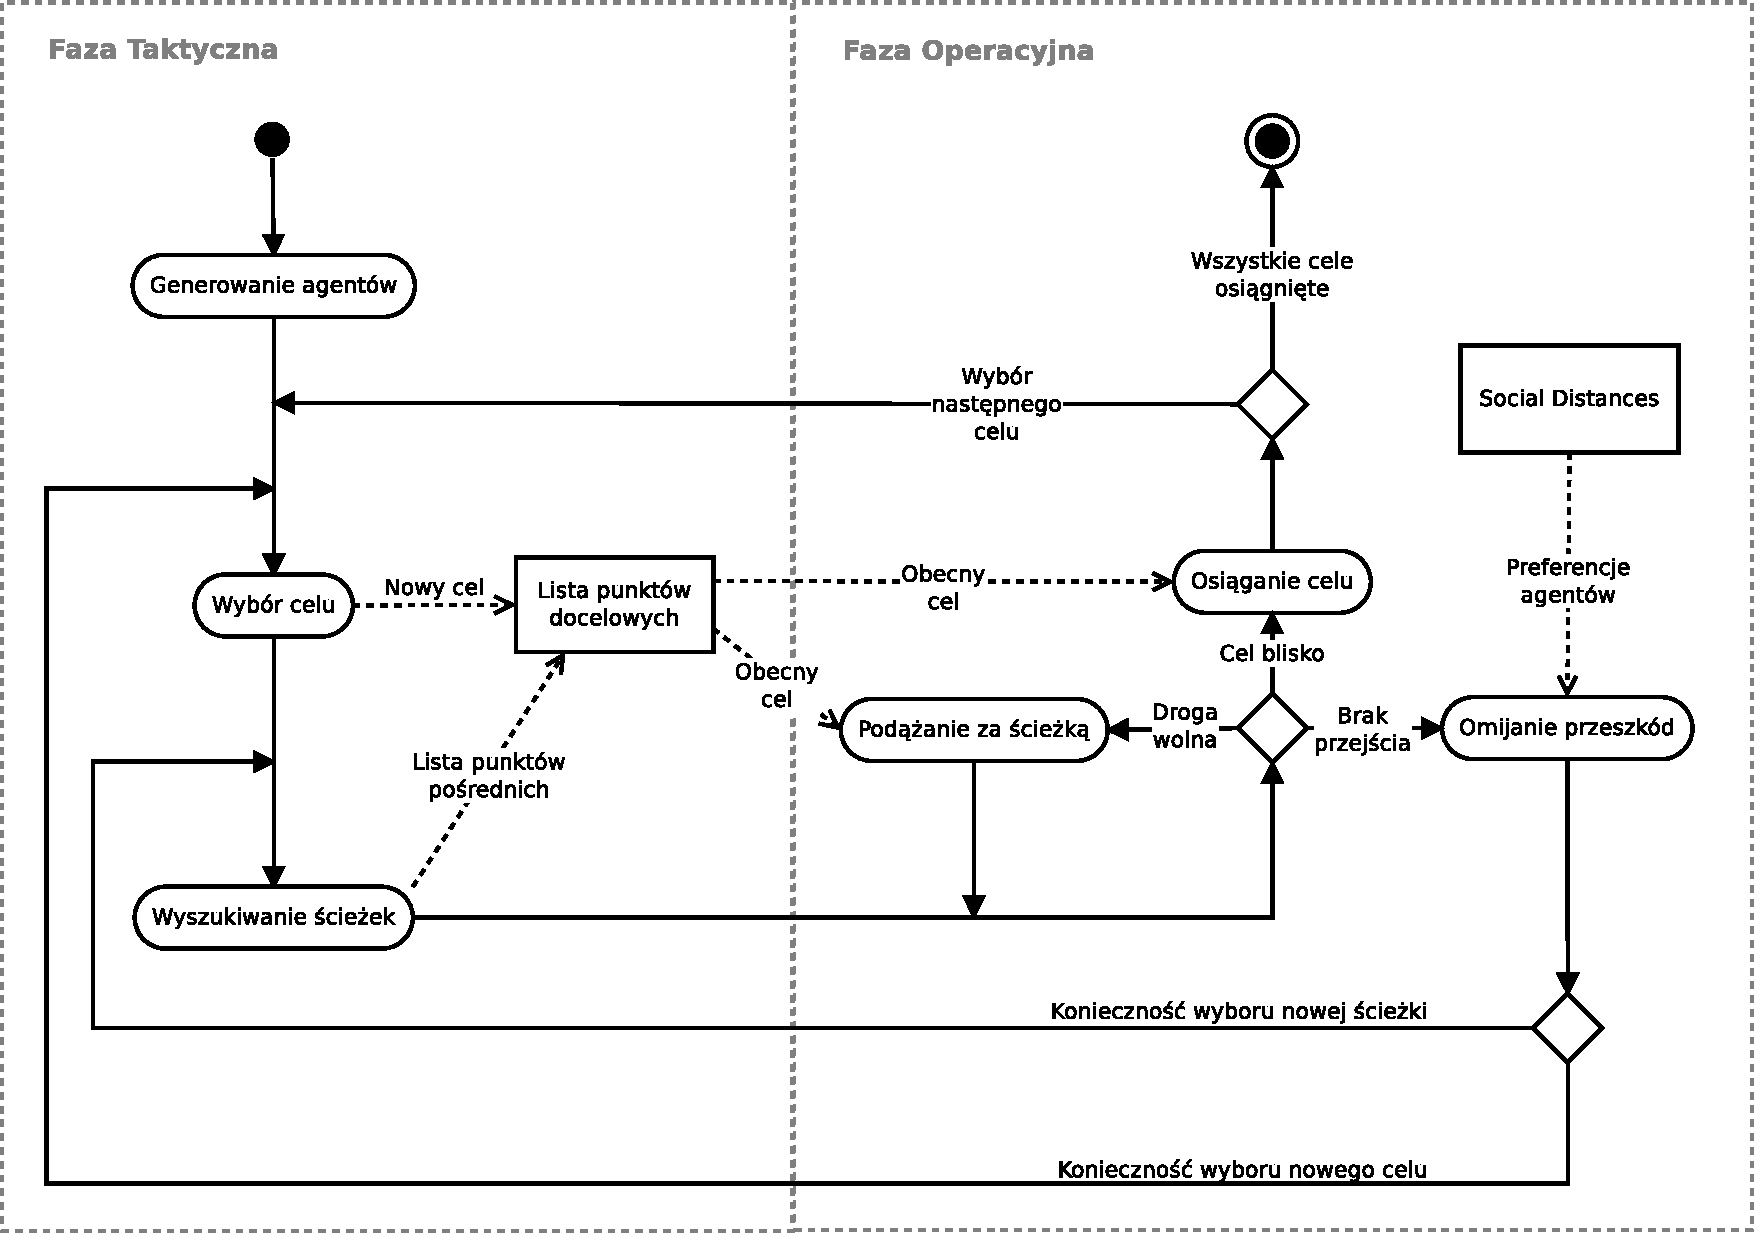
\includegraphics[scale=0.55]{./img/ActorActivity.pdf}
	\caption{Diagram aktywno�ci agent�w.}
	\label{fig:actor-activity}
\end{figure}

Ka�dy agent generowany jest na podstawie jednego z predefiniowanych archetyp�w, kt�ry okre�la jego predyspozycje fizyczne oraz zachowanie (np. maksymaln� pr�dko�� ruchu, sk�onno�� do zmiany pasa ruchu itp.).

Nast�pnie dla ka�dego agenta wybierana jest wst�pna lista miejsc docelowych, kt�re zamierza on odwiedzi�, oraz obliczana zostaje optymalna �cie�ka ��cz�ca poszczeg�lne miejsca z listy. �cie�ka ta zostaje zmodyfikowana w oparciu o map� rozk�adu stref specjalnych tak, aby wierniej oddawa� faktyczne zamiary danego agenta. Faza taktyczna ko�czy si� wybraniem pewnej niewielkiej ilo�ci punkt�w po�rednich le��cych na wyznaczonej �cie�ce - ma to na celu u�atwienie agentowi odnalezienie w�a�ciwej drogi.

Po wygenerowaniu niezb�dnych danych taktycznych przechodzi do fazy operacyjnej, w kt�rej nast�puje w�a�ciwe przemieszczanie agent�w. W tej fazie dla ka�dego z agent�w rozpatrywane s� takie zachowania jak omijanie przeszk�d, grupowanie si� i pod��anie za obran� �cie�k� - na podstawie danych z ich lokalnego otoczenia. W przypadku osi�gni�cia miejsca docelowego agent zaczyna przemieszcza� si� w kierunku kolejnego z zaplanowanych cel�w b�d� przechodzi w tryb "`b��dzenia"', gdy osi�gnie ostatni z wyznaczonych cel�w.

%---------------------------------------------------------------------------

\section{Faza taktyczna}
\label{sec:tactical}

Faza taktyczna ma na celu oddanie og�lnych zamiar�w ka�dego z klient�w co do wizyty w centrum handlowym - wyboru miejsc docelowych oraz obrania drogi prowadz�cej po kolei do ka�dego z nich. Oznacza to, �e zachodzi ona globalnie dla ka�dego z agent�w. W fazie taktycznej uwzgl�dnieny jest tylko rozk�ad potencjalnych cel�w (w tym mapa \hyperref[sec:mall-impl]{stref specjalnych}), tzn. takie czynniki jak po�o�enie innych agent�w (nawet gdy blokuj� korytarz) nie s� brane pod uwag� przy wyznaczaniu �cie�ek (Rys. \ref{fig:tactical}).

�cie�ki ruchu obliczane s� za pomoc� algorytmu \hyperref[sec:path-finding]{A*}. Mapa rozk�adu stref specjalnych centrum handlowego jest wykorzystywana jako dodatkowa heurystyka A* - strefy specjalne modyfikuj� szacowan� ocen� danego punktu nale��cego do wyznaczanej �cie�ki, nadaj�c jej po��dany kszta�t i prowadz�c j� w odpowiedni spos�b do celu podr�y.

Przy wyznaczaniu �cie�ek brane s� pod uwag� r�wnie� \hyperref[sec:attractors]{atraktory}, \hyperref[sec:queues]{kolejki} i \hyperref[sec:entrance-exits]{przej�cia}, kt�re algorytm stara si� uwzgl�dni� z pomoc� opisanej heurystyki.

\begin{figure}[h]
	\centering
	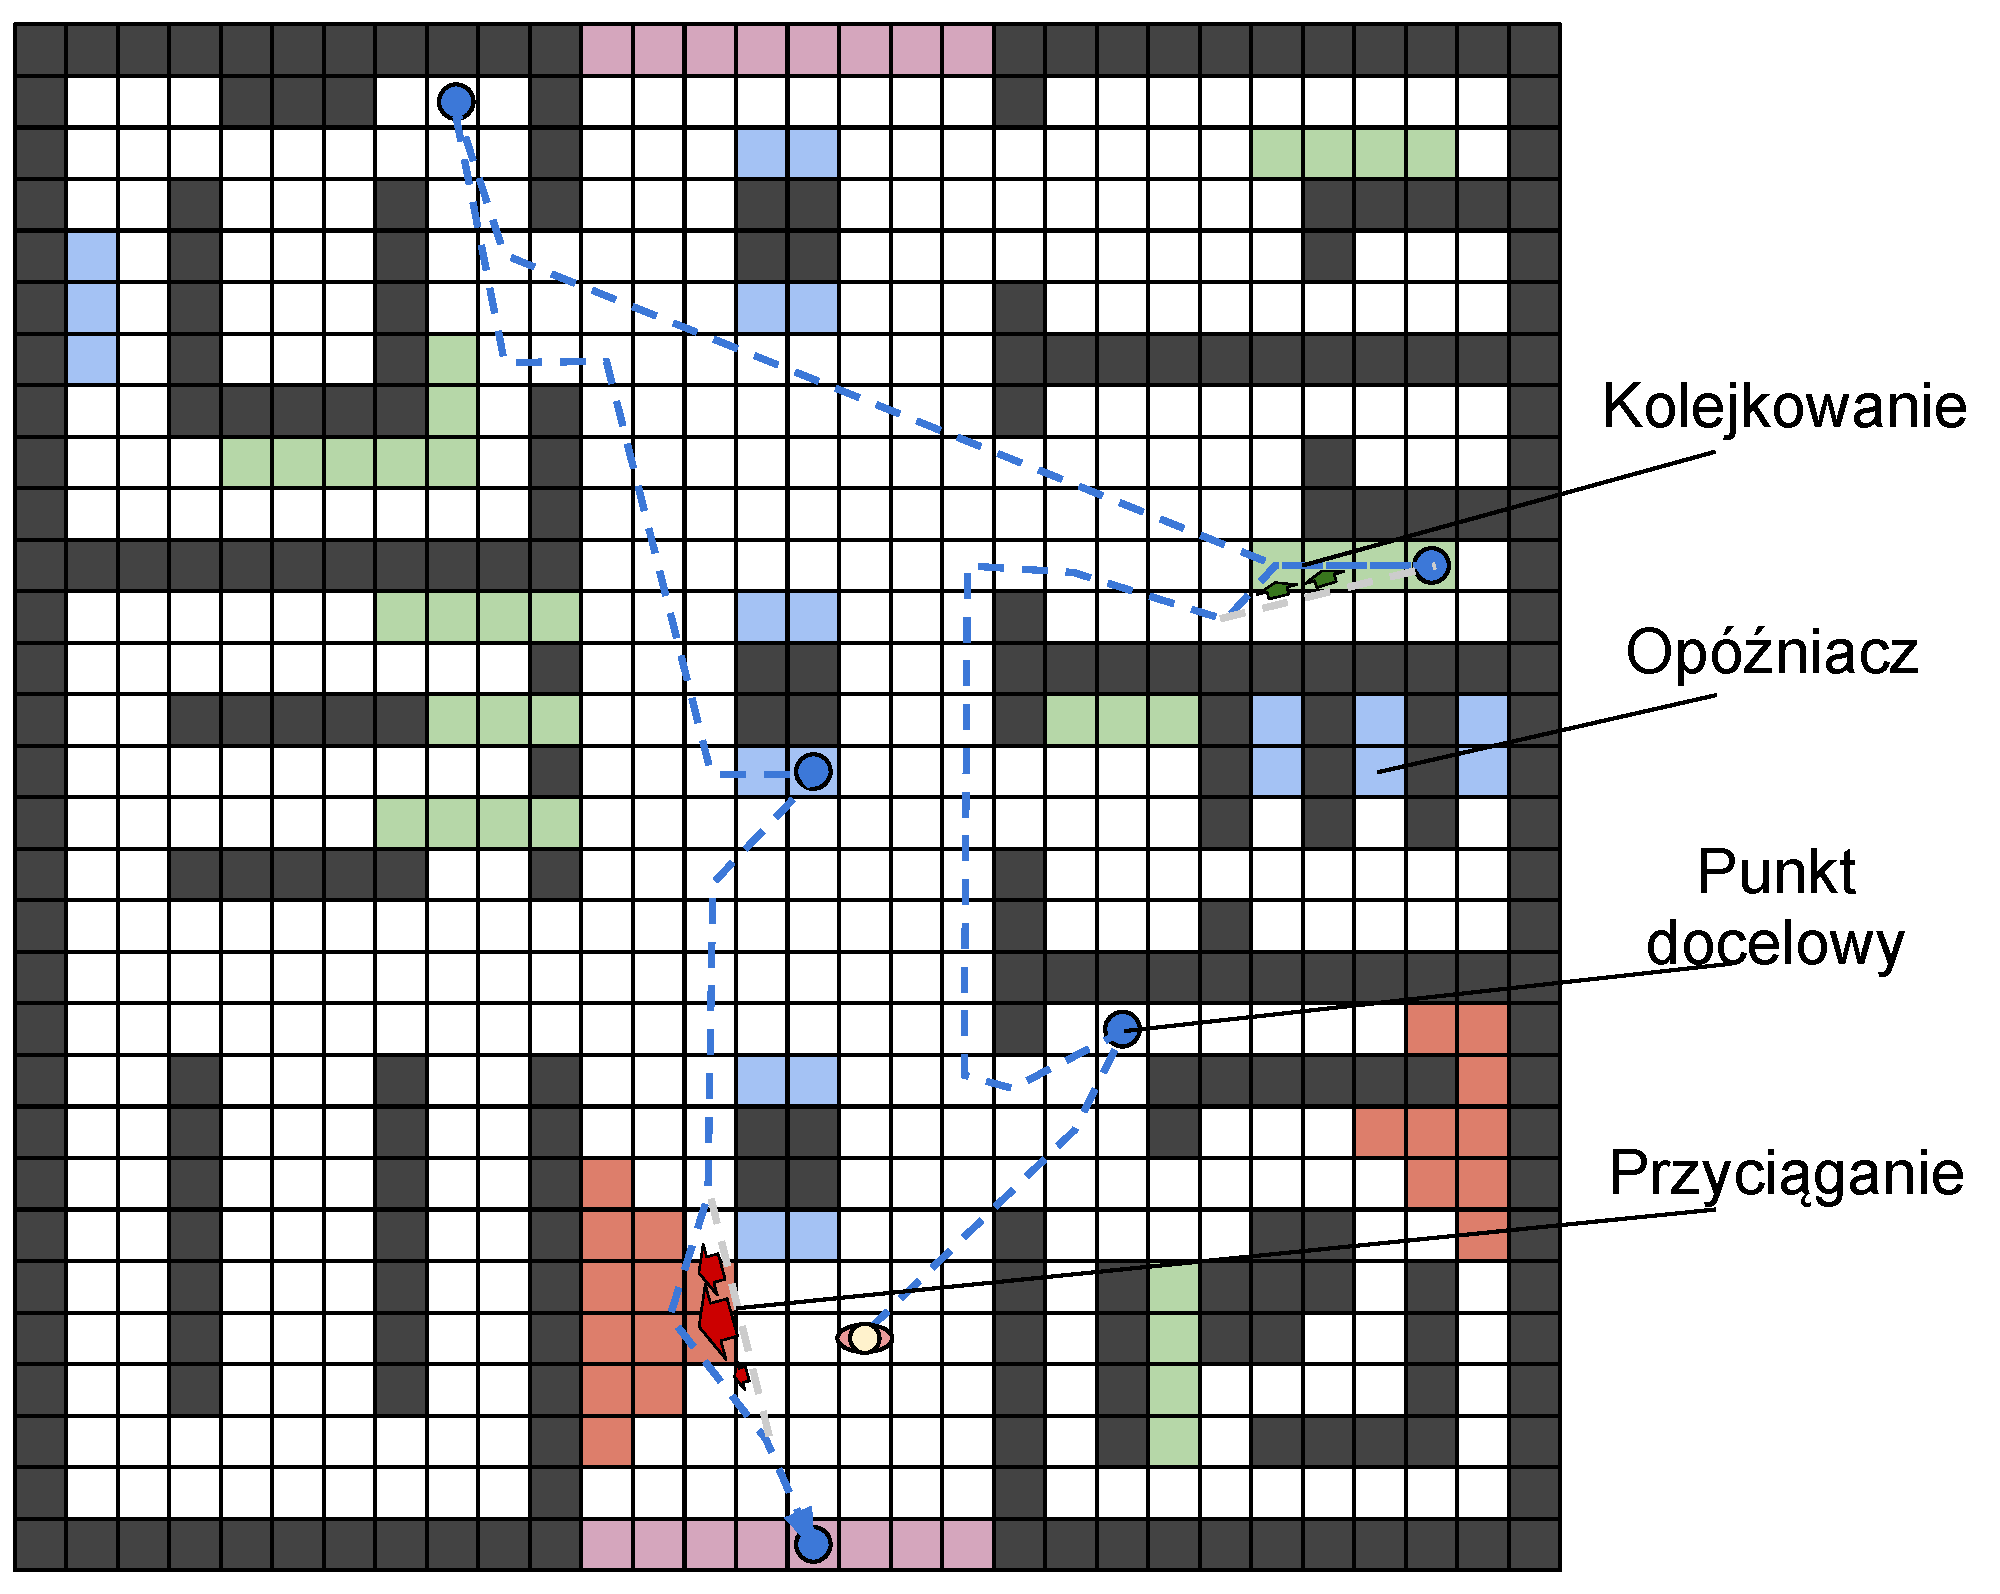
\includegraphics[scale=0.3]{./img/Tactical.pdf}
	\caption{Zakres dzia�ania taktycznej cz�ci modelu ruchu.}
	\label{fig:tactical}
\end{figure}

%---------------------------------------------------------------------------

\section{Faza operacyjna}
\label{sec:operational}

% TODO Potrzeba wi�kszego opisu, kt�ry bardziej zag��bia si� w wybrany algorytm operacyjny.

W fazie operacyjnej dla ka�dego agenta zostaje podj�ta decyzja o jego dalszym ruchu na podstawie danych z jego lokalnego otoczenia (Rys. \ref{fig:operational}) . W szczeg�lno�ci rozpatrywane s� warianty unikni�cia ewentualnej kolizji z innymi agentami b�d� przeszkodami - w tym celu zastosowano zmodyfikowane algorytmy \hyperref[sec:movement-impl]{Ped-4} oraz \hyperref[sec:social-force-impl]{Social Distances}.
W niniejszej symulacji pierwszy z nich u�ywany jest do modelowania ruchu ludzi w alejkach i korytarzach (gdy� prowadzi on do samoorganizowania si� potok�w pieszych w tzw. pasy ruchu), natomiast s�u�y do opisania ruchu pieszych na placach (gdzie generalnie ka�dy posiada mo�liwo�� swobodnego omijania innych).

\begin{figure}[h]
	\centering
	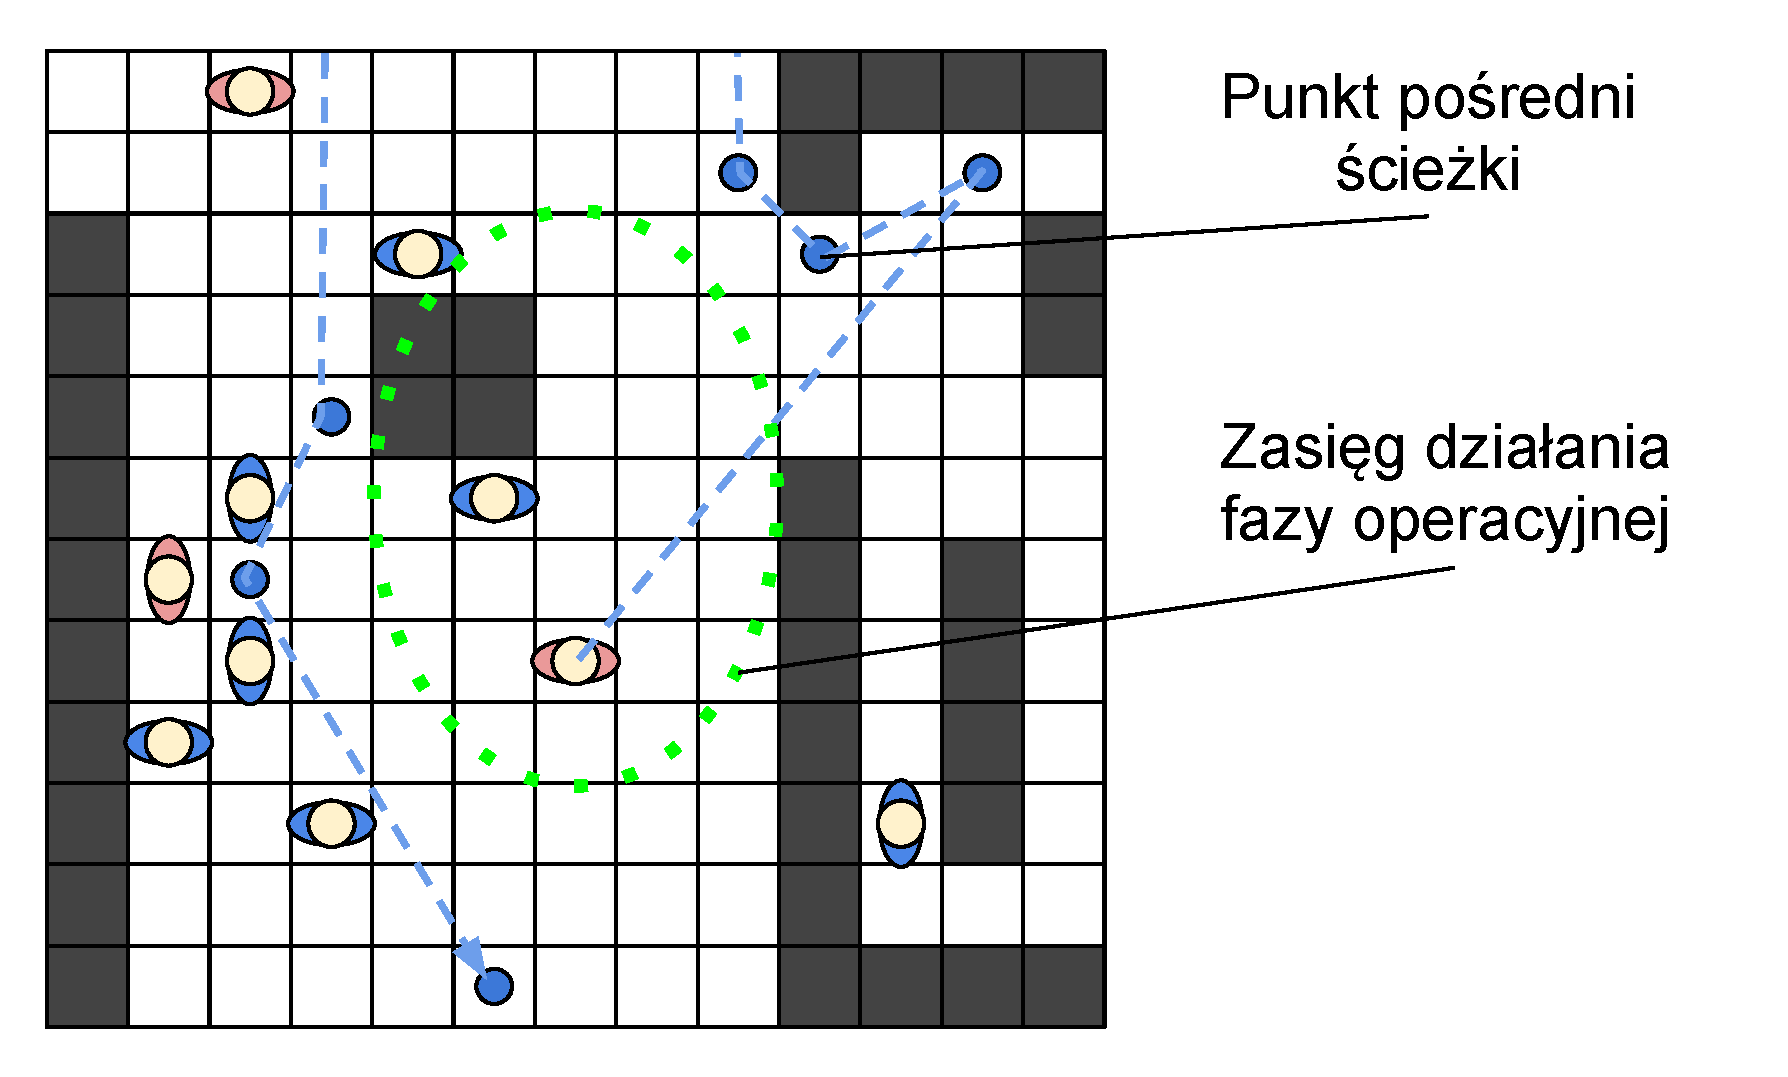
\includegraphics[scale=0.3]{./img/Operative.pdf}
	\caption{Zakres dzia�ania operacyjnej cz�ci modelu ruchu.}
	\label{fig:operational}
\end{figure}

Algorytm \textbf{Ped-4} sk�ada si� z nast�puj�cych etap�w:
\begin{enumerate}
\item \textbf{Dostosowanie kierunku ruchu} \
    - gdy k�t mi�dzy kierunkiem ruchu, a kierunkiem do celu przekroczy warto�� graniczn�, pieszy skr�ca w stron� celu.
\item \textbf{Zmiana pasa ruchu} \
    - obliczana jest ilo�� wolnych p�l dla obecnie zajmowanego pasa i dla pas�w s�siednich. Pieszy zajmuje ten pas, kt�ry na chwil� obecn� umo�liwia mu przesuni�cie si� o najwi�ksz� ilo�� p�l do przodu. Przy wyborze preferowany jest dotychczasowy pas. W przypadku, gdy obecnie zajmowany pas nie jest "`czysty"' (tzn. z naprzeciwka idzie inny pieszy), aby unikna� kolizji pieszy stara si� "`schowa�"' za inn� osob� id�c� w tym samym co on kierunku.
\item \textbf{Krok naprz�d} \
    - w przypadku, gdy pole bezpo�rednio przed pieszym (zgodnie z kierunkiem ruchu) jest wolne - pr�ba zaj�cia go. Je�li nie jest to mo�liwe - pr�ba dokonania zamiany miejsca z innym pieszym. Wymiana odzwierciedla sytuacj�, gdy piesi "`skr�caj� tu�owie"', by "`przecisn�� si�"' obok siebie. Etap \textit{krok naprz�d} powtarzany jest wielokrotnie, dop�ki nie sko�cz� si� "`punkty ruchu"' pieszego.
\end{enumerate}

Poni�ej zamieszczono preferowan� kolejno�� dokonywania zamian:

\begin{enumerate}
	\item mi�dzy pieszymi id�cymi w przeciwnych kierunkach na tym samym pasie
	\item mi�dzy pieszymi id�cymi w przeciwnych kierunkach na s�siednich pasach (na polach po przek�tnej)
	\item mi�dzy pieszymi id�cymi w kierunkach prostopad�ych wzgl�dem siebie (na polach po przek�tnej)
	\item mi�dzy pieszymi id�cymi w kierunkach prostopad�ych wzgl�dem siebie (jeden "`tarasuje"' drugiemu drog�)
\end{enumerate}

Pieszy mo�e wybra� dan� mo�liwo�� tylko wtedy, gdy jego "`partner"' do zamiany nie wykona� jeszcze swojego ruchu. Je�li dana wymiana nie dojdzie do skutku, pr�bowana jest kolejna opcja z listy (znajduje to potwierdzenie w obserwacjach - w sytuacji du�ego t�oku ludzie ch�tniej dokonuj� takich manewr�w).

Zaproponowany przez W�sa i in. model \textbf{Social Distances} \cite{social-distance-agh} opiera si� na obserwacji, �e ka�dy cz�owiek posiada wok� siebie (g��wnie przed sob�) tzw. \textit{stref� komfortu}, kt�rej naruszenie przez inne osoby prowadzi do dyskomfortu. Oznacza to, �e agenci b�d� porusza� si� w taki spos�b, by w mo�liwie jak najmniejszym stopniu narusza� nawzajem swoje strefy komfortu. Aby to osi�gn�� na podstawie obszaru poszczeg�lnych stref wyznaczany zostaje swoisty rozk�ad potencja�u, przy czym maj�c do wyboru kilka mo�liwych p�l agenci przemieszczaj� si� na pole o najmniejszym potencjale. Je�li w danym momencie brak jest dost�pnych p�l, pieszy "`drepcze"' w miejscu w oczekiwaniu na zwolnienie si� kt�rego� z nich.

%\chapter{Model centrum handlowego}
\label{cha:mall-model}

Na model centrum handlowego sk�ada si� zar�wno opis jego geometrii (tj. przebieg �cian, rozk�ad wej�� i wyj��), jak r�wnie� rozk�ad stref specjalnych, kt�re w swego rodzaju aktywny spos�b wp�ywaj� na zachowanie pieszych - mowa o \emph{atraktorach}, \emph{kolejkach} i \emph{miejscach oczekiwania}. Umo�liwiaj� one symulujacj� takich zachowa�, jak \emph{grupowanie si�} czy \emph{kolejkowani} poprzez modyfikacj� domy�lnego algorytmu ruchu fazy taktycznej. Istnienie stref specjalnych stwierdzono do�wiadczalnie na podstawie obserwacji ruchu ludzi w Galerii Krakowskiej.

Wszystkie powy�sze elementy zilustrowano na rys. \ref{fig:overview}.

\begin{figure}[h]
	\centering
	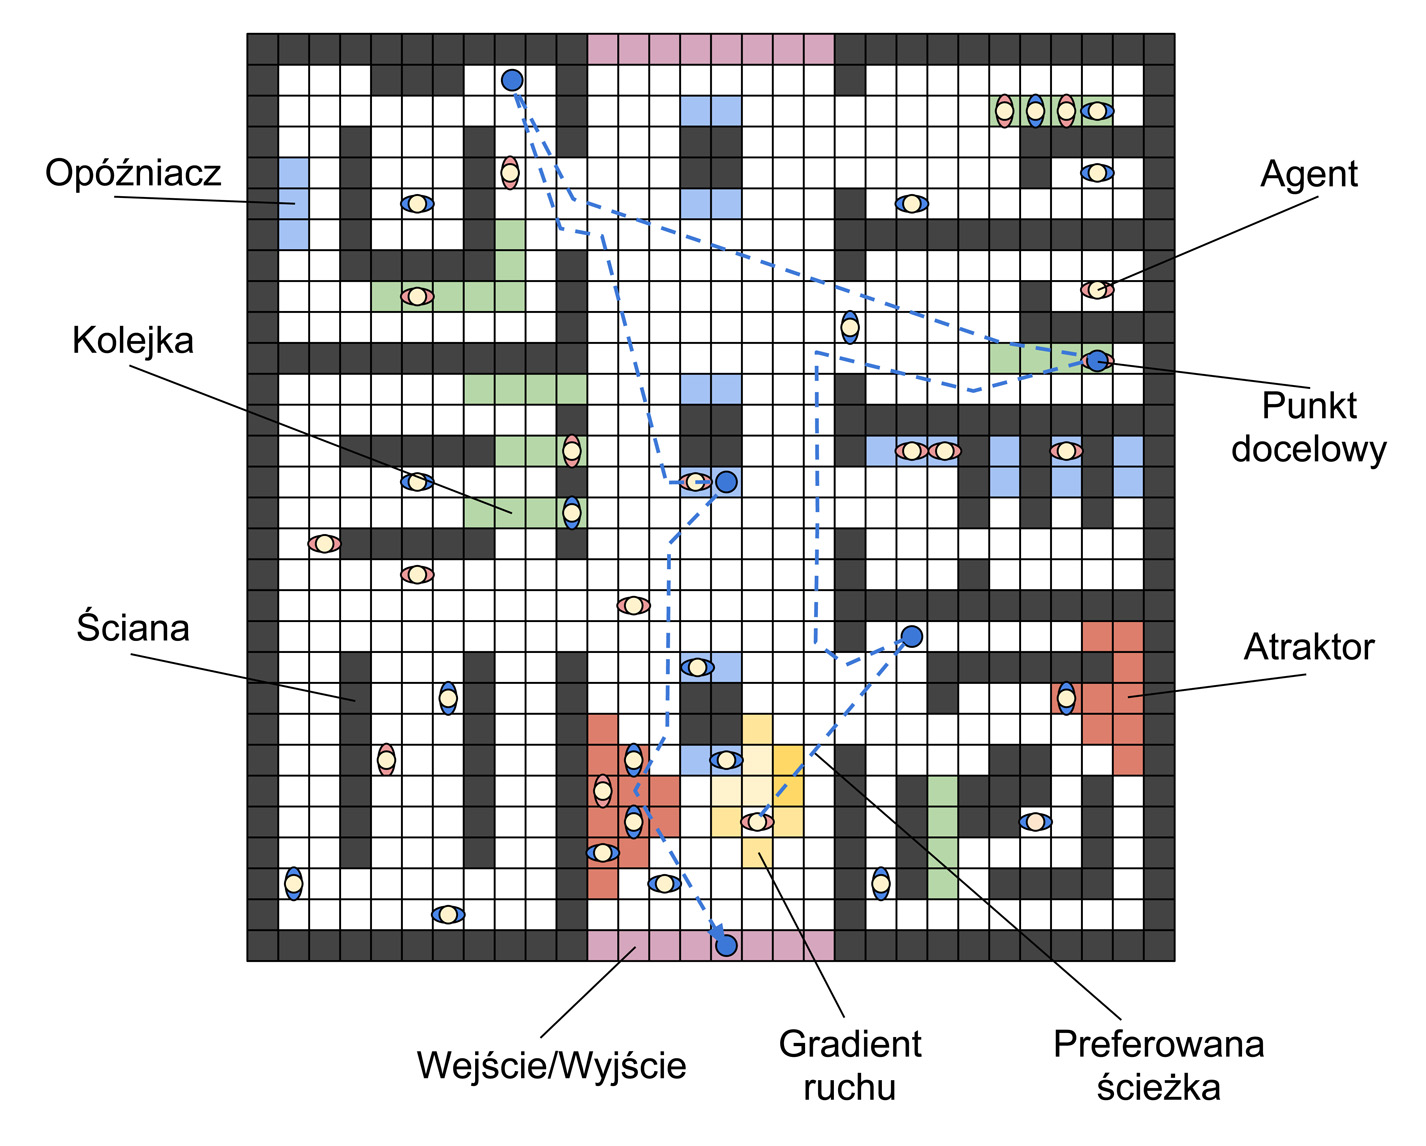
\includegraphics[scale=0.3]{./img/Overview.jpg}
	\caption{Zastosowana dekompozycja problemu.}
	\label{fig:overview}
\end{figure}

%---------------------------------------------------------------------------

\section{Atraktor}
\label{sec:attractors}

Atraktor ma za zadanie modelowa� obecno�� przedmiotu lub zjawiska, kt�re przykuwa uwag� ludzi na terenie centrum handlowego, a wynikiem jego dzia�ania jest spontaniczne powstawanie skupisk ludzi, tzw. grupowanie si� (Rys. \ref{fig:crowding}). Atraktory r�ni� si� mi�dzy sob� typami, a r�ne typy przyci�gaj� uwag� r�nego rodzaju agent�w, co odzwierciedla r�nice w preferencjach ludzi przebywaj�cych w centrum handlowym. W wi�kszo�ci przypadk�w atraktor nie wyst�puje pojedynczo, lecz tworzy strefy, w kt�rych wyr�ni� mo�na �r�d�o zjawiska przyci�gaj�cego uwag� o radialnym gradiencie spadku si�y przyci�gania.

Dzia�anie atraktora opiera si� na modyfikowaniu szacowanego kosztu ruchu dla danej p�ytki wykorzystywanego p�niej przez algorytm A*.

\begin{figure}[h]
	\centering
	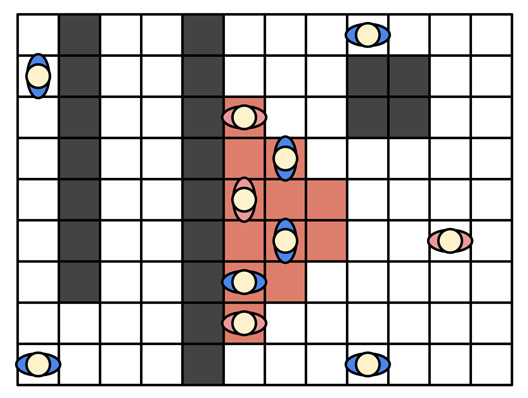
\includegraphics[scale=0.4]{./img/Crowding.jpg}
	\caption{Grupowanie si� agent�w w obr�bie atraktora.}
	\label{fig:crowding}
\end{figure}

%---------------------------------------------------------------------------

\section{Kolejka}
\label{sec:queues}

Strefa kolejki s�u�y modelowaniu zjawiska \emph{�cis�ego kolejkowania si�} ludzi (na przyk�ad przy kasie sklepowej lub na stopniach schod�w ruchomych), co nie wynika z og�lnego modelu ruchu (Rys. \ref{fig:queueing}).

Kolejka to w zasadzie ci�g atraktor�w tak silnie oddzia�uj�cych na pieszych, �e po wej�ciu na jedno z p�l kolejki dalszy ruch mo�liwy jest tylko na kolejne z jej p�l. Dodatkowo pola kolejki powoduj� zatrzymanie agenta na danej p�ytce na pewn� ilo�� cykli symulacji, co oddaje okres oczekiwania na obs�u�enie.

\begin{figure}[h]
	\centering
	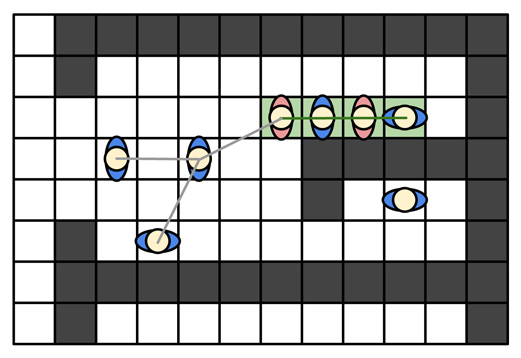
\includegraphics[scale=0.4]{./img/Queueing_model.jpg}
	\caption{Kolejkowanie si� ludzi przy kasie sklepowej z zaznaczon� kolejk� �cis��.}
	\label{fig:queueing}
\end{figure}

%---------------------------------------------------------------------------

\section{Przej�cia}
\label{sec:passages}

Strefy przej�cia modeluj� ci�gi komunikacyjne prowadz�ce bezpo�rednio do przej�� pomi�dzy pi�trami centrum handlowego - klatek schodowych, schod�w ruchomych, wind itp. (Rys. \ref{fig:passing-through}).

W obr�bie strefy przej��, podobnie jak w przypadku kolejek, modyfikowane s� preferencje odleg�o�ciowe agent�w (innymi s�owy zmienia si� wp�yw naruszania strefy komfortu na ruch agenta), dzi�ki czemu mo�liwe jest zmniejszenie odleg�o�ci mi�dzy pieszymi, co nie wynika z og�lnego modelu ruchu.

\begin{figure}[h]
	\centering
	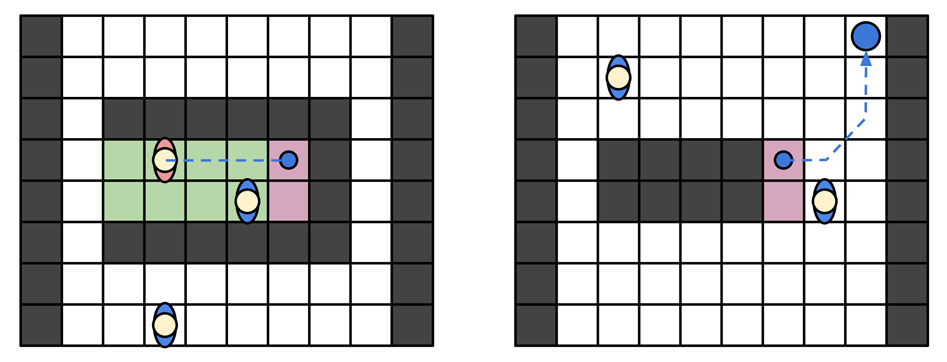
\includegraphics[scale=0.4]{./img/EntranceExits.jpg}
	\caption{Poruszanie si� agenta po schodach ruchomych pomi�dzy pi�trami centrum handlowego.}
	\label{fig:passing-through}
\end{figure}

%---------------------------------------------------------------------------

\section{Wej�cia/wyj�cia}
\label{sec:entrance-exits}

Wej�cia i wyj�cia to jedyne miejsca, w kt�rych mo�e pojawi� si� nowy agent - klient centrum handlowego - oraz jedyne miejsca, w kt�rych mo�e on zako�czy� swoj� wizyt� w centrum handlowym.

%---------------------------------------------------------------------------

\section{Miejsca oczekiwania}
\label{sec:holders}

Miejsce oczekiwania odzwierciedla takie obiekty centrum handlowego, jak �aweczki b�d� stoliki - miejsca, w kt�rych klienci przysiadaj� i sp�dzaj� pewien okres czasu w bezruchu.

Dzia�anie miejsca oczekiwania polega na zatrzymaniu wszelkiej aktywno�ci agenta na okres pewnej liczby cykli symulacji.

\begin{figure}[h]
	\centering
	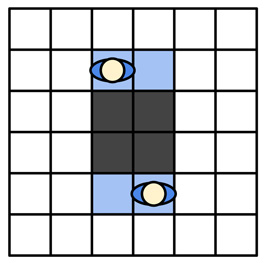
\includegraphics[scale=0.4]{./img/Held.jpg}
	\caption{Klienci centrum odpoczywaj�cy na �awce.}
	\label{fig:held-down}
\end{figure}

%---------------------------------------------------------------------------

\section{Uwagi}
\label{sec:notes}

Nale�y zaznaczy�, �e na chwil� obecn� potencja� niekt�rych z element�w modelu centrum handlowego nie zosta� w pe�ni wykorzystany. Przyk�adem wi�kszej integracji stref specjalnych z modelem ruchu mog�yby by� uwzgl�dnienie potrzeb os�b starszych do robienia cz�stych odpoczynk�w poprzez dodawanie miejsca oczekiwania - �awki - do cel�w podr�y (we w miar� regularnych odst�pach czasu).
\newpage
    \section{Implementacja}
    \label{sec:implementation}

    W celu wykonania projektu pos�u�ono si� j�zykiem \textbf{Java} oraz bibliotekami \textbf{Java Swing} oraz \href{http://www.randelshofer.ch/monte/}{\textbf{Monte Media Library}}. Poni�ej zawarto opis implementacji wybranych algorytm�w i obiekt�w symulacji.

        \subsection{Reprezentacja centrum handlowego}
        \label{sec:mall-impl}

        Centra handlowe reprezentowane s� za pomoc� map bitowych (plik�w \emph{.bmp}), kt�rych piksele koduj� odpowiadaj�ce im kom�rki siatki symulacji, co pozwala tworzy� nowe rozk�ady pomieszcze� i stref spejcalnych w bardzo prosty i szybki spos�b. Implementacja przewiduje istnienie dw�ch map dla ka�dego centrum handlowego - map� rozk�adu pomieszcze� i algorytm�w ruchu fazy operacyjnej (rysunek \ref{fig:mall-layout}) oraz map� rozk�adu stref specjalnych centrum handlowego (rysunek \ref{fig:mall-features}).

        \begin{figure}[H]
            \centering
            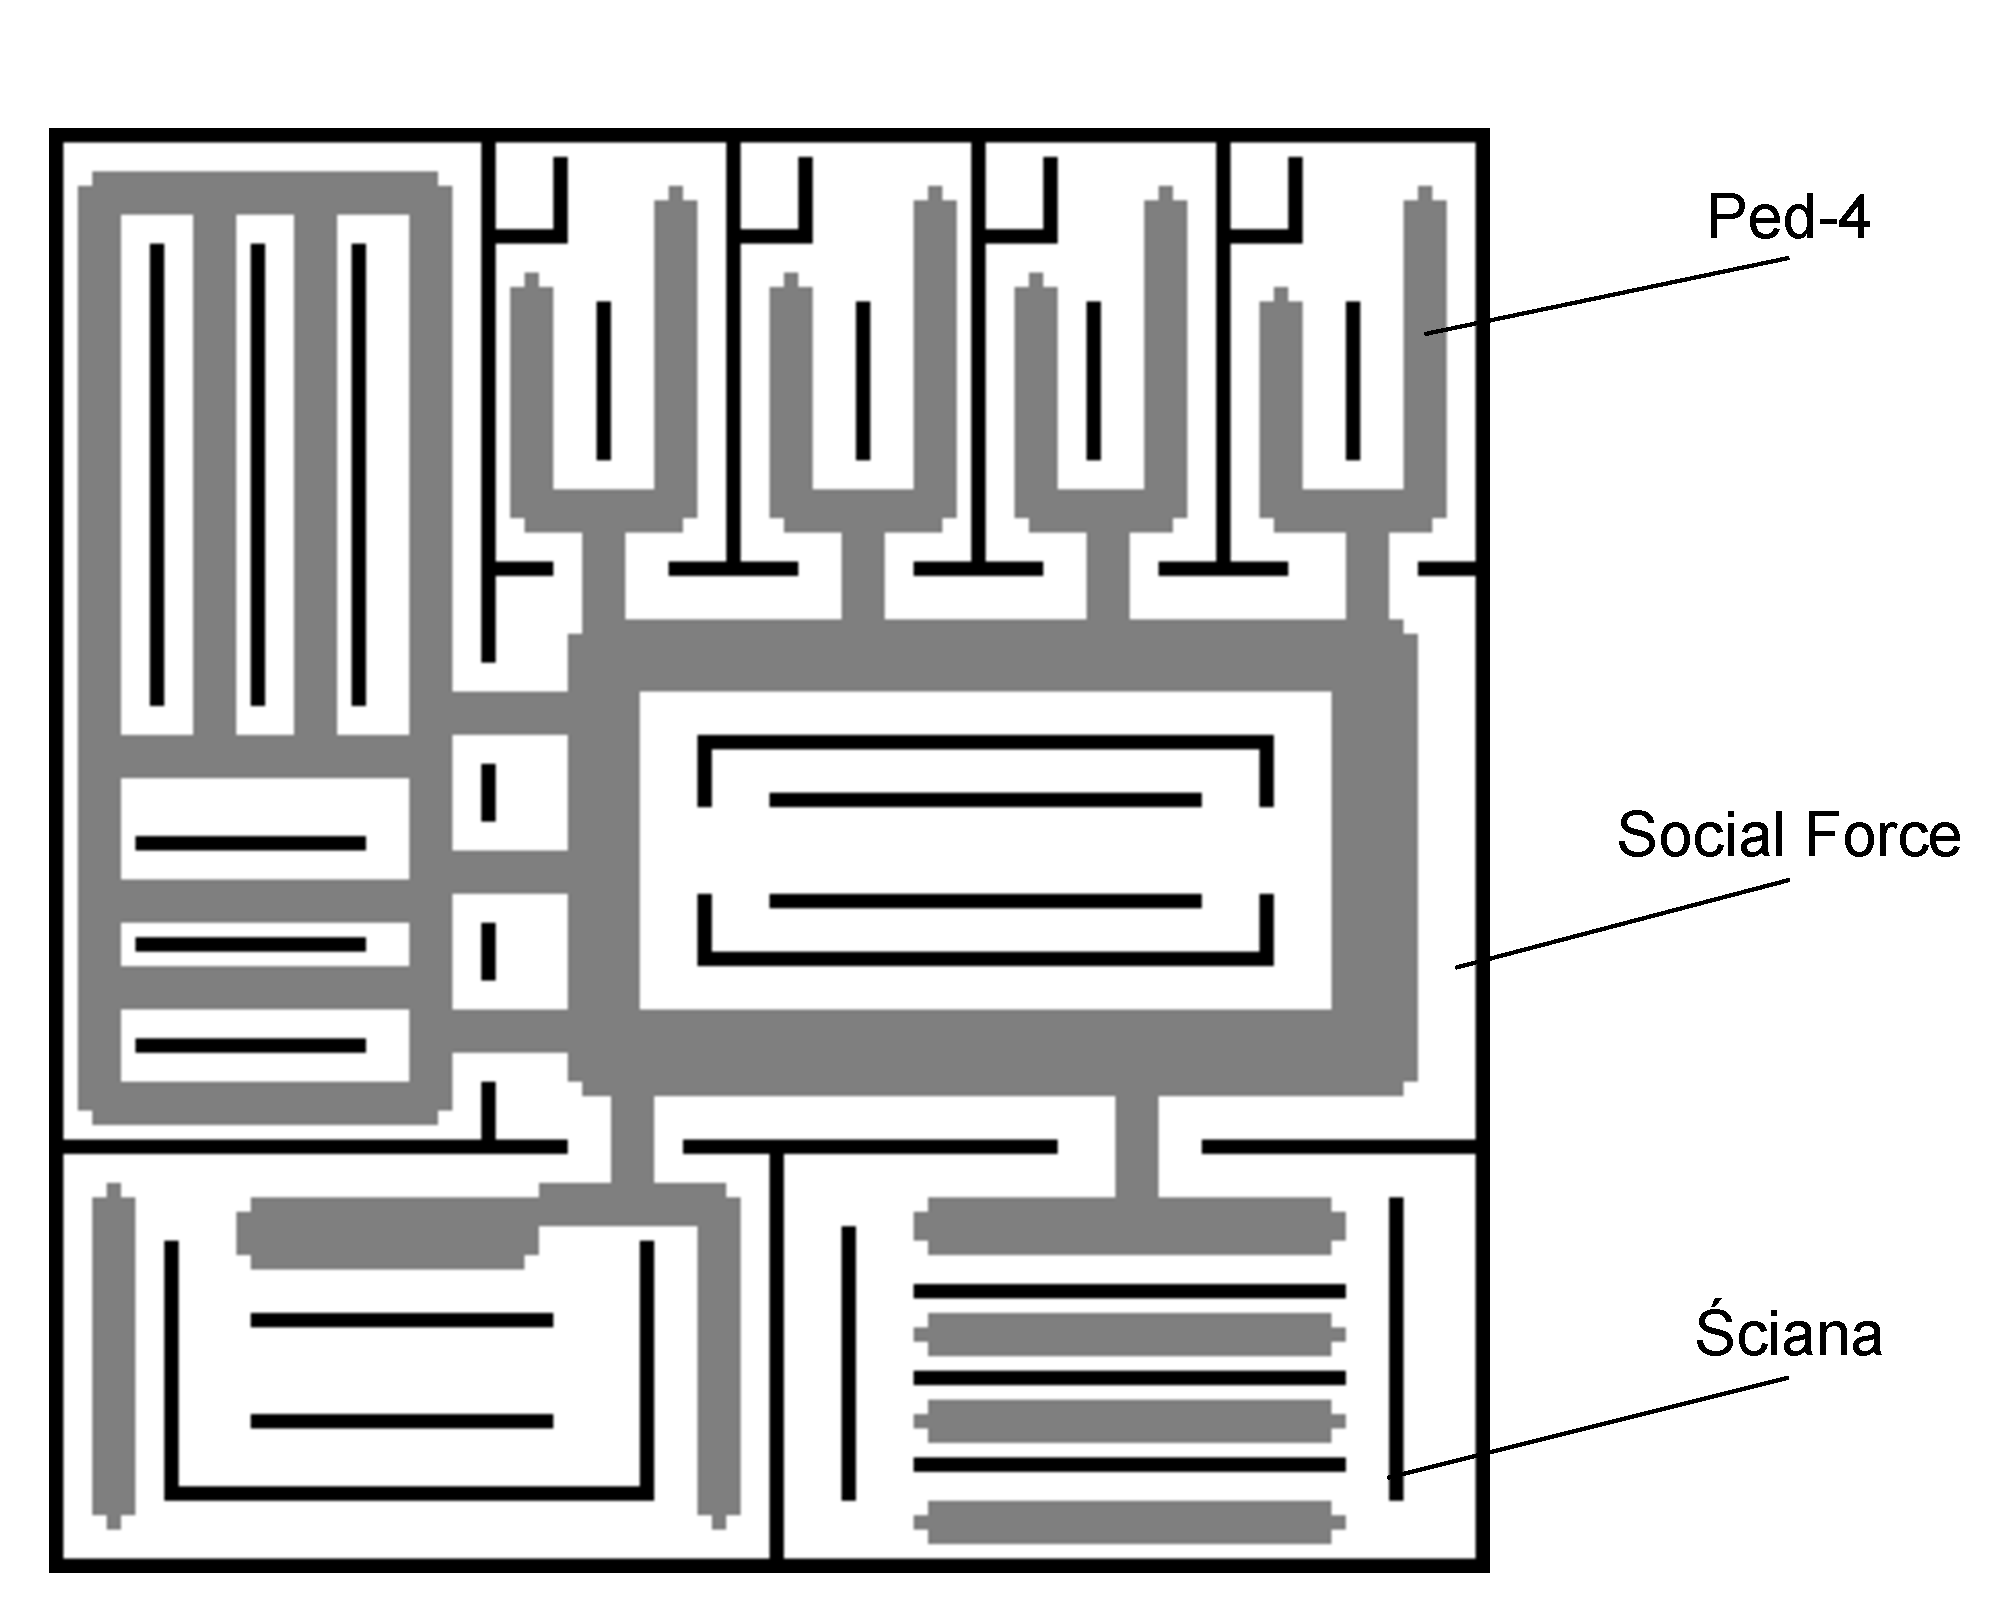
\includegraphics[scale=0.3]{./img/MallLayout.pdf}
            \caption{Przyk�adowy rozk�ad pomieszcze� i algorytm�w ruchu ma�ego centrum handlowego.}
            \label{fig:mall-layout}
        \end{figure}

        \emph{Mapa rozk�adu pomieszcze�} zawiera informacje o fizycznych w�a�ciwo�ciach pomieszcze� modelowanego centrum handlowego - usytu��wanie �cia� i innych obiekt�w blokuj�cych przej�cie. Dodatkowo zawarto na niej rozk�ad algorytm�w ruchu wykorzystanych w \hyperref[sec:operational]{fazie operacyjnej}, co pozwala jednoznacznie okre�li� po�o�enie korytarzy, skrzy�owa� i innych cech centrum handlowego zwi�zanych z ruchem agent�w. \\

\noindent
Warto�ci znacz�ce poszczeg�lnych pixeli $RGB$ mapy:

        \begin{itemize}
            \item $(0x00, *, *)$ - warto�� zarezerwowana dla �cian i innych obiekt�w blokuj�cych przej�cie.
            \item $(0x7F, *, *)$ - warto�� determinuj�ca wykorzystanie algorytmu \hyperref[sec:movement-impl]{Ped-4}.
            \item $(0xFF, *, *)$ - warto�� determinuj�ca wykorzystanie algorytmu \hyperref[sec:social-force-impl]{Social Force}.
        \end{itemize}

        \begin{figure}[H]
            \centering
            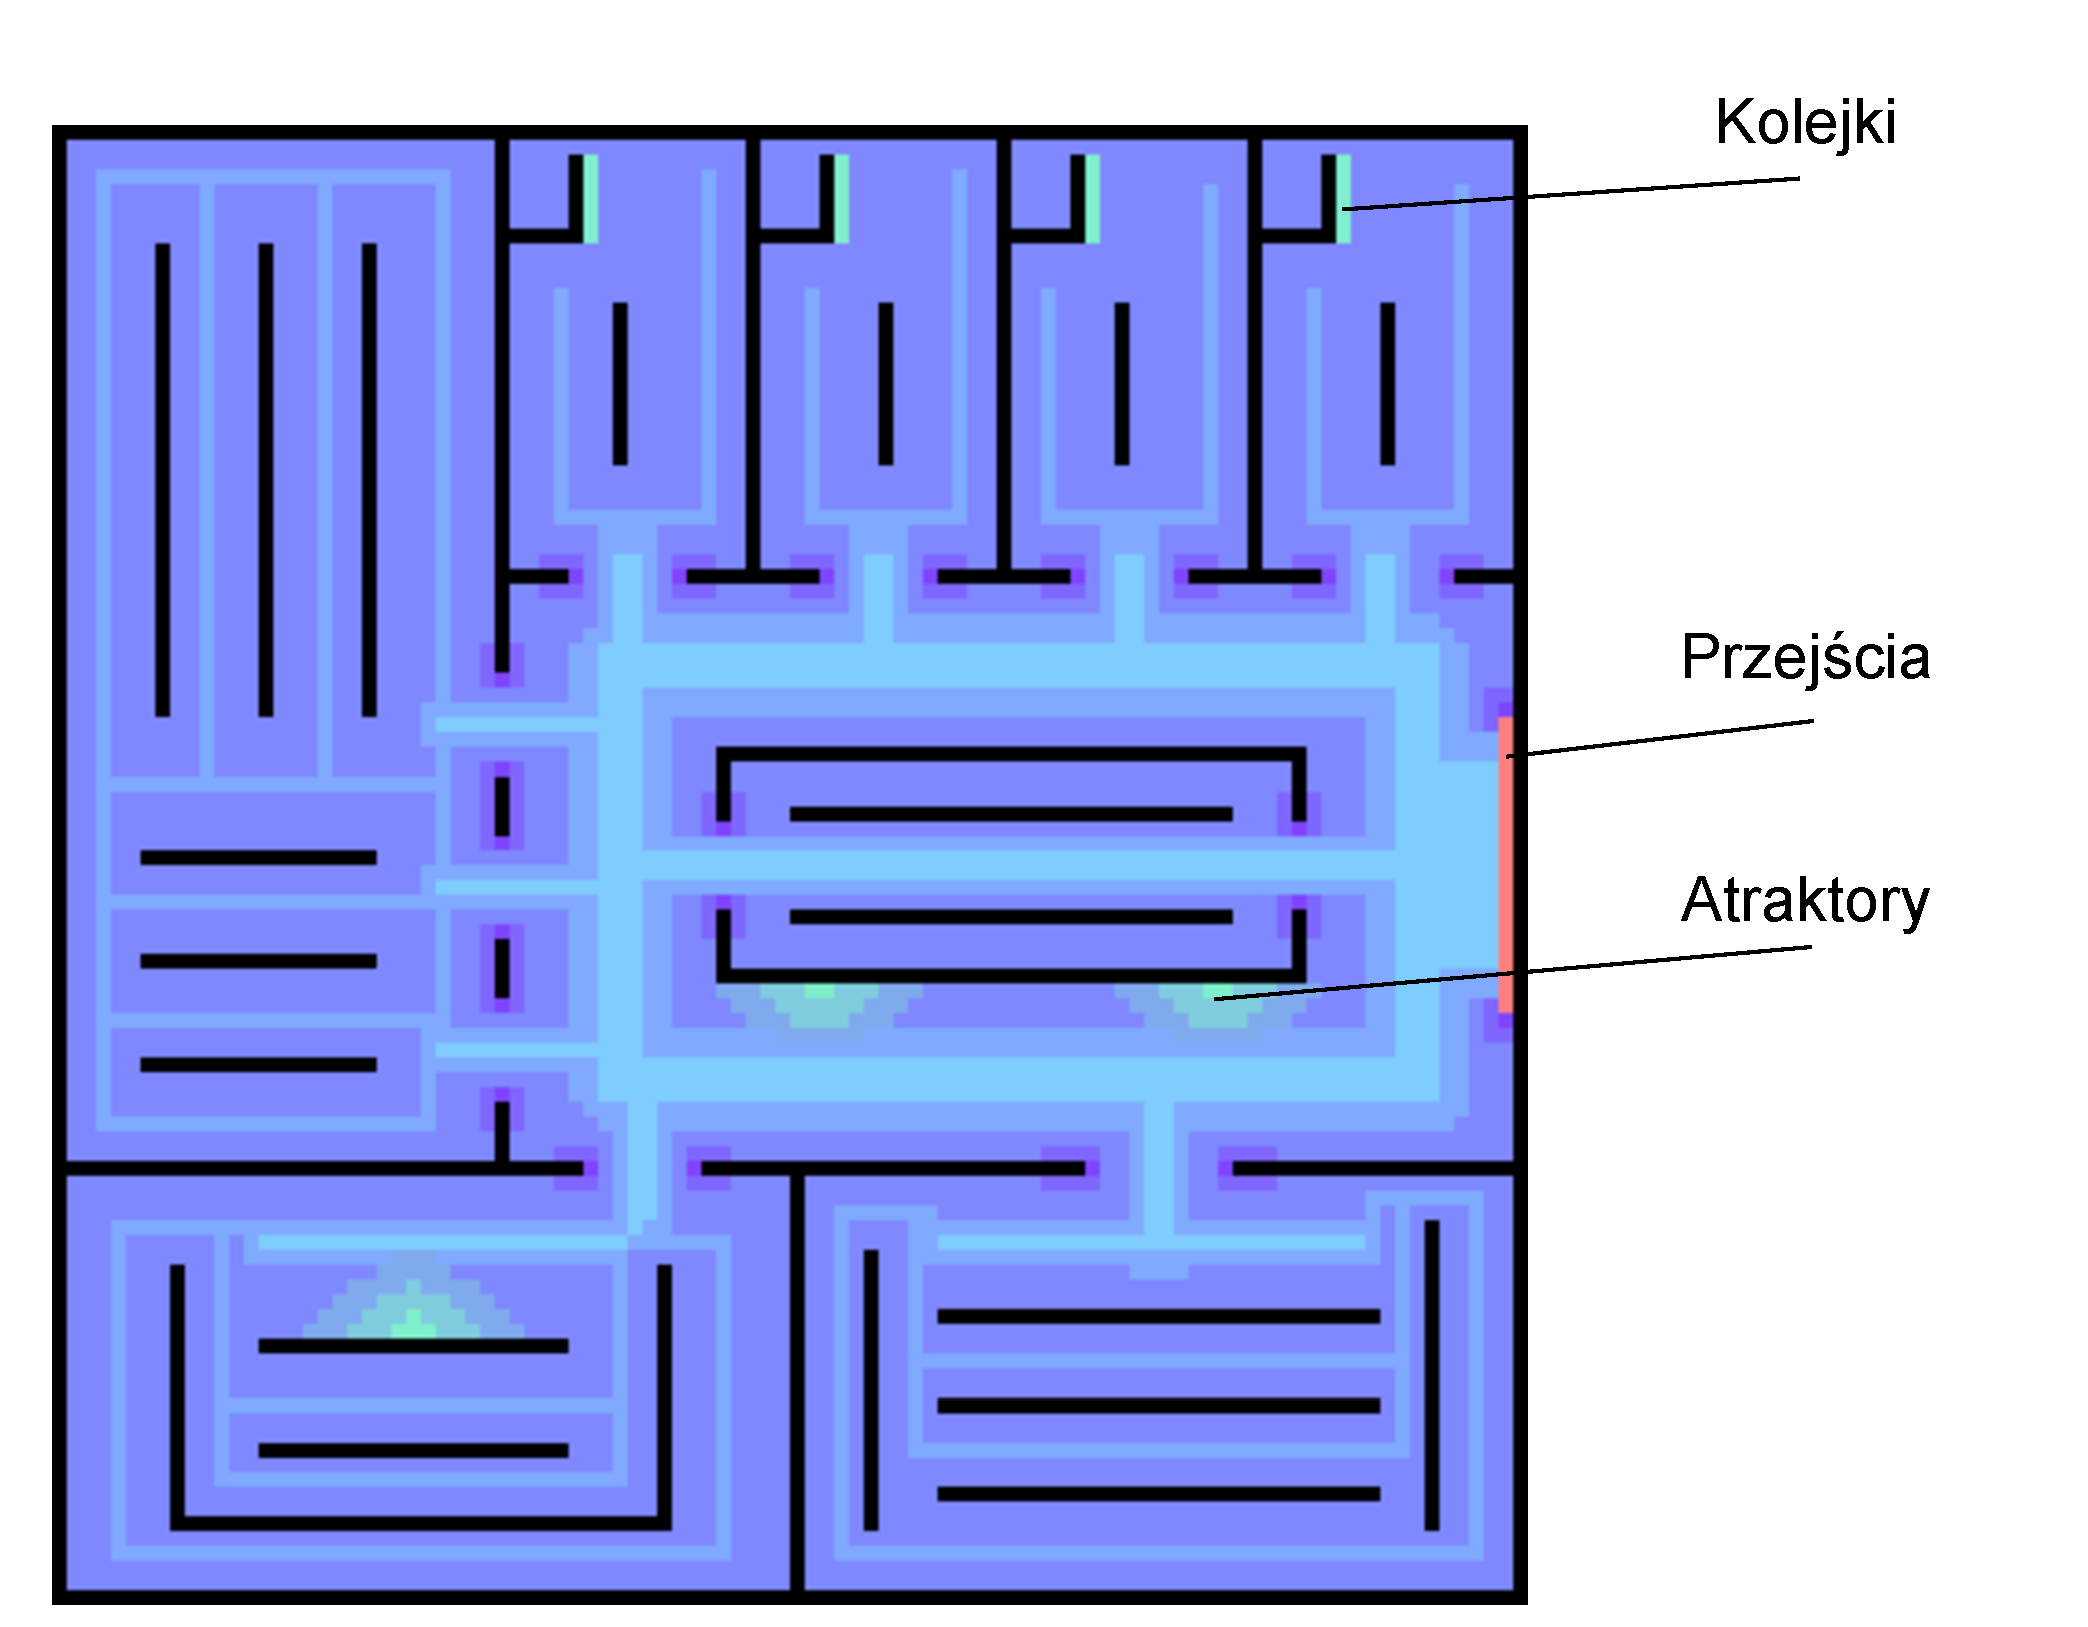
\includegraphics[scale=0.3]{./img/MallFeatures.pdf}
            \caption{Przyk�adowy rozk�ad stref specjalnych ma�ego centrum handlowego.}
            \label{fig:mall-features}
        \end{figure}

        \emph{Mapa rozk�adu stref specjalnych} centrum handlowego zawiera informacje o funkcjonalnych cechach modelowanego centrum handlowego - rozmieszczenie miejsc przeznaczonych do czekania, kolejek przy kasach sklepowych, okien wystawowych i sieci routingu u�atwiaj�cej przemieszczanie si� w centrum handlowym. Informacje te wykorzystywane s� przede wszystkim przez \hyperref[sec:tactical]{faz� taktyczn�} wykorzystanego algorytmu, gdzie s� s�u�� jako \hyperref[sec:path-deviation]{dodatkowa heurystyka} \hyperref[sec:path-finding]{algorytmu wyszukiwania �cie�ek A*}. \\

\noindent
Warto�ci znacz�ce poszczeg�lnych pixeli $RGB$ mapy:

        \begin{itemize}
            \item $(0x7F, A, H)$ - warto�� oznaczaj�ca \hyperref[sec:path-deviation]{uog�lniony atraktor} o \emph{atrakcyjno�ci} $A$ i \emph{czasie wstrzymania} $H$.
            \item $(0xFF, *, *)$ - warto�� oznaczaj�ca \hyperref[sec:entrance-exits]{przej�cia/wej�cia}, kt�re odpowiednio tworz� lub usuwaj� agent�w z symulacji.
        \end{itemize}

\noindent
Z racji ograniczonego czasu i ni�szego priorytetu implementacja nie uwzgl�dnia istnienia wielu pi�ter w centrum handlowym - symulacja ruchu ludzi wewn�trz wielopi�trowego centrum handlowego mo�e by� traktowana jako wiele symulacji ruchu ludzi wewn�trz jednopi�trowego centrum handlowego.

        \subsection{Wyb�r puntk�w docelowych}
        \label{sec:destination-choice}

        \emph{Punkty docelowe} reprezentuj� cele podr�y agent�w. Z racji mniejszego priorytetu i braku czasu algorytm wybiera zadan� ilo�� losowych miejsc znajduj�cych si� we wn�trzu centrum handlowego, kt�re nast�pnie sortuje celem minimalizacji sumarycznej d�ugo�ci drogi je ��cz�cej. Opisany spos�b wyboru miejsc docelowych pozwala symulowa� wszystkie zachowania poruszaj�cych si� ludzi na poziomie lokalnym (na przyk�ad kolejkowanie si�) i wi�kszo�� schemat�w zachowa� t�umu na poziomie globalnym (z wy��czeniem bardziej abstrakcyjnych zachowa� uwarunkowanych socjologicznie i kulturowo, takich jak r�ne stosunki ilo�ciowe agent�w danego typu w r�nych cz�ciach centrum handlowego).

\newpage
        \subsection{Znajdowanie �cie�ek}
        \label{sec:path-finding}

W celu wyznaczania �cie�ek prowadz�cych do punkt�w docelowych wykorzystano algorytm \textbf{A*}. A* jest algorytmem kompletnym, s�u��cym do wyznaczania najkr�tszej drogi ��cz�cej dwa wierzcho�ki grafu, kt�ry w ka�dym przypadku jest w stanie znale�� drog�, je�li takowa istnieje. A* wykorzystuje \hyperref[sec:path-deviation]{heurystyk�}, kt�ra estymuje koszt �cie�ki prowadz�cej z danego wierzcho�ka do celu, staraj�c si� rozpatrywa� tylko najbardziej obiecuj�ce wierzcho�ki. \\

\noindent
Algorytm przochowuje zbiory wierzcho�k�w ``otwartych'' i ``zamkni�tych'', czyli odpowiednio, wierzcho�k�w, kt�re s� rozpatrywane i tych, kt�re ju� zosta�y sprawdzone. Dzia�anie algorytmu rozpoczyna si� od dodania aktualnej pozycji agenta do zbioru wierzcho�k�w otwartych. W ka�dym nast�pnym kroku algorytm wykonuje iteracyjnie nast�puj�ce operacje:

        \begin{itemize}
            \item Ze zbioru wierzcho�k�w otwartych wybierany jest najbardziej obiecuj�cy wierzcho�ek $x$, minimalizuj�cy funkcj� $f(x)$:
              \[ f(x) = g(x) + h(x) \]
              gdzie $g(x)$ okre�la d�ugo�� drogi prowadz�cej z wierzcho�ka pocz�tkowego do wierzcho�ka $x$, a $h(x)$ okre�la przewidywan� przez heurystyk� d�ugo�� drogi ��cz�cej wierzcho�ek $x$ i cel podr�y.
            \item W przypadku osi�gni�cia punktu docelowego algorytm ko�czy si� sukcesem.
            \item W przeciwnym przypadku wierzcho�ek $x$ dodawany jest do zbioru wierzcho�k�w zamikni�tych, a s�siaduj�ce z nim wierzcho�ki (wierzcho�ki osi�galne w jednym kroku zaczynaj�c w $x$), kt�re nie nale�� do zbioru wierzcho�k�w zamkni�tych, dodawane s� do zbioru wierzcho�k�w otwartych.
        \end{itemize}

\noindent
Zale�nie od zastosowanej heurystyki algorytm A* jest w stanie dostarcza� optymalne �cie�ki ��cz�ce dwa punkty lub suboptymalne �cie�ki, kt�re s� obliczane szybciej. Ze wzgl�du na rozwi�zywany problem i brak wymogu dostarczania optymalnych �cie�ek w implementacji zastosowano z�o�on�, dopuszczaln� (\emph{ang. admissible}) heurystyk� opisan� w nast�pnej sekcji, kt�r� dodatkowo obarczono wag� $\epsilon = 5$, co pozwala szybko generowa� �cie�ki o po��danym i koszcie nie przekraczaj�cym $\epsilon$ razy kosztu �cie�ki optymalnej.

        \subsection{Dewiacja �cie�ek}
        \label{sec:path-deviation}

        Dewiacja �cie�ek zachodzi podczas dzia�ania algorytmu wyszukiwania �cie�ek opisanego w poprzedniej sekcji celem u�atwienia zachodzenia pewnych zachowa�, takich jak poruszanie si� w odpowiedni spos�b po korytarzach centrum handlowego. Odpowiednia dewiacja �cie�ek zosta�a osi�gni�ta przez modyfikacj� heurystyki zastosowanego algorytmu A* - ka�dy fragment \hyperref[fig:mall-features]{mapy rozk�adu stref specjalnych} centrum handlowego posiada przypisan� mu warto�� determinuj�c� parametry \textbf{uog�lnionego atraktora} - \emph{atrakcj� A} oraz \emph{czas wstrzymania H}. \\

        \emph{Atrakcja} odpowiada za przyci�ganie agent�w do pewnych stref centrum handlowego i ma za zadanie przede wszystkim umo�liwi� realizacj� zdefiniowanych przy analizie problemu \hyperref[sec:attractors]{atraktor�w}. Jej warto�� kodowana jest przez komponent $G$ pixeli $RGB$ mapy rozk�adu stref specjalnych centrum handlowego, koduj�cych atraktory (komponent $R$ r�wny $0x7F$). Warto�� komponentu $G$ nale�y podzieli� przez $0x7F$ celem przeskalowania do przedzia�u $[0, 2)$. Heurystyka algorytmu A* wykorzystuje t� warto��, jako dodatkowy mno�nik estymowanego kosztu �cie�ki, tote� warto�� 0 oznacza najsilniejsz� atrakcj�, warto�� 1 brak atrakcji natomiast warto�� 2 oznacza odpychanie - algorytm wyszukiwania �cie�ek b�dzie preferowa� inne drogi.

        \emph{Czas wstrzymania} odpowiada za op�nianie agent�w podczas wykonywania ruchu - agent osi�gaj�cy kom�rk� siatki symulacji obarczon� czasem oczekiwania zostaje op�niony na zadan� ilo�� czasu. Warto�� czasu wstrzymania kodowana jest przez komponent $B$ pixeli $RGB$ mapy rozk�adu stref specjalnych centrum handlowego, koduj�cych atraktory. Warto�� tego komponentu traktowana jest jako ilo�� krok�w symulacji, na kt�re op�niany agent zostanie wstrzymany. \\

Implementacja \emph{uog�lnionego atraktora} okaza�a si� na tyle elastyczna, �e wyeliminowa�a konieczno�� osobnej implementacji \hyperref[sec:queues]{kolejek} i \hyperref[sec:holders]{op�niaczy} - kolejki realizowane s� jako linie znacz�co zwi�kszonej atrakcji o kr�tkim czasie wstrzymania, natomiast op�niacze s� punktami o znacz�co zwi�kszonym czasie wstrzymania. \hyperref[sec:attractors]{Atraktory} zosta�y zrealizowane jako gradienty zwi�kszaj�cej si� atrakcji i czasu wstrzymania - agenci odwiedzajacy atraktor sp�dzaj� w nim tym wi�cej czasu, im bli�ej jego centrum si� znajduj�. Dodatkowym atutem zastosowanej implementacji jest mo�liwo�� routingu agent�w w centrum handlowym. Wszystkie formy stref specjalnych wyra�onych przez modyfikacj� heurystyki algorytmu A* zosta�y zawarte na pogl�dowym rysunku \ref{fig:mall-features}.

        \subsection{Reprezentacja agent�w}
        \label{sec:actor-impl}

        Na chwil� obecn� agenci opisywani s� przez parametry wp�ywaj�ce tylko i wy��cznie na ich ruch w fazie operacyjnej. Docelowo planowane jest rozszerzenie ich zachowania o preferencje dotycz�ce odwiedzanych miejsc, czasu sp�dzanego w galerii itp.

    \begin{figure}[H]
        \centering
        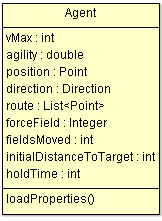
\includegraphics[scale=0.75]{./img/agent.png}
        \caption{Klasa agenta}
        \label{fig:agent}
    \end{figure}

\noindent
Znaczenie poszczeg�lnych parametr�w:
\begin{itemize}
\item \textbf{vMax} – maksymalna ilo�� punkt�w ruchu do wykorzystania w danej iteracji fazy operacyjnej
\item \textbf{agility} – sk�onno�� do dokonywania zamian z innymi podczas etapu poruszania agent�w
\item \textbf{position} – po�o�enie agenta na planszy galerii
\item \textbf{direction} – aktualny kierunek ruchu (dost�pne kierunki s� zgodne ze stronami �wiata)
\item \textbf{route} – lista wsp�rz�dnych p�ytek-cel�w do odwiedzenia
\item \textbf{forceField} – opis warto�ci potencja�u p�l wok� agenta (przy za�o�eniu, �e agent zwr�cony jest w kierunku p�nocnym)
\item \textbf{fieldsMoved} – odleg�o�� (mierzona w p�ytkach) przebyta od ostatniego celu do danej chwili
\item \textbf{initialDistanceToTarget} – teoretyczna minimalna odleg�o�� od poprzedniego do obecnego celu
\item \textbf{holdTime} – pozosta�y czas oczekiwania (np. w kolejce)
\end{itemize}

Cz�� spo�r�d powy�szych parametr�w agenta inicjalizowana jest na podstawie plik�w zawieraj�cych opisy pewnych og�lnych charakterystyk ludzi, np. "typ dynamiczny" oznacza cz�owieka poruszaj�cego si� szybko i sk�onnego do dokonywania zamian, "typ emeryta" oznacza stateczny krok i niech�� do zamian.

        \subsection{Ruch agent�w i Ped-4}
        \label{sec:movement-impl}

\noindent
Faza operacyjna sk�ada si� z czterech wykonywanych w p�tli etap�w, co zilustrowano na poni�szym schemacie:

    \begin{figure}[H]
        \centering
        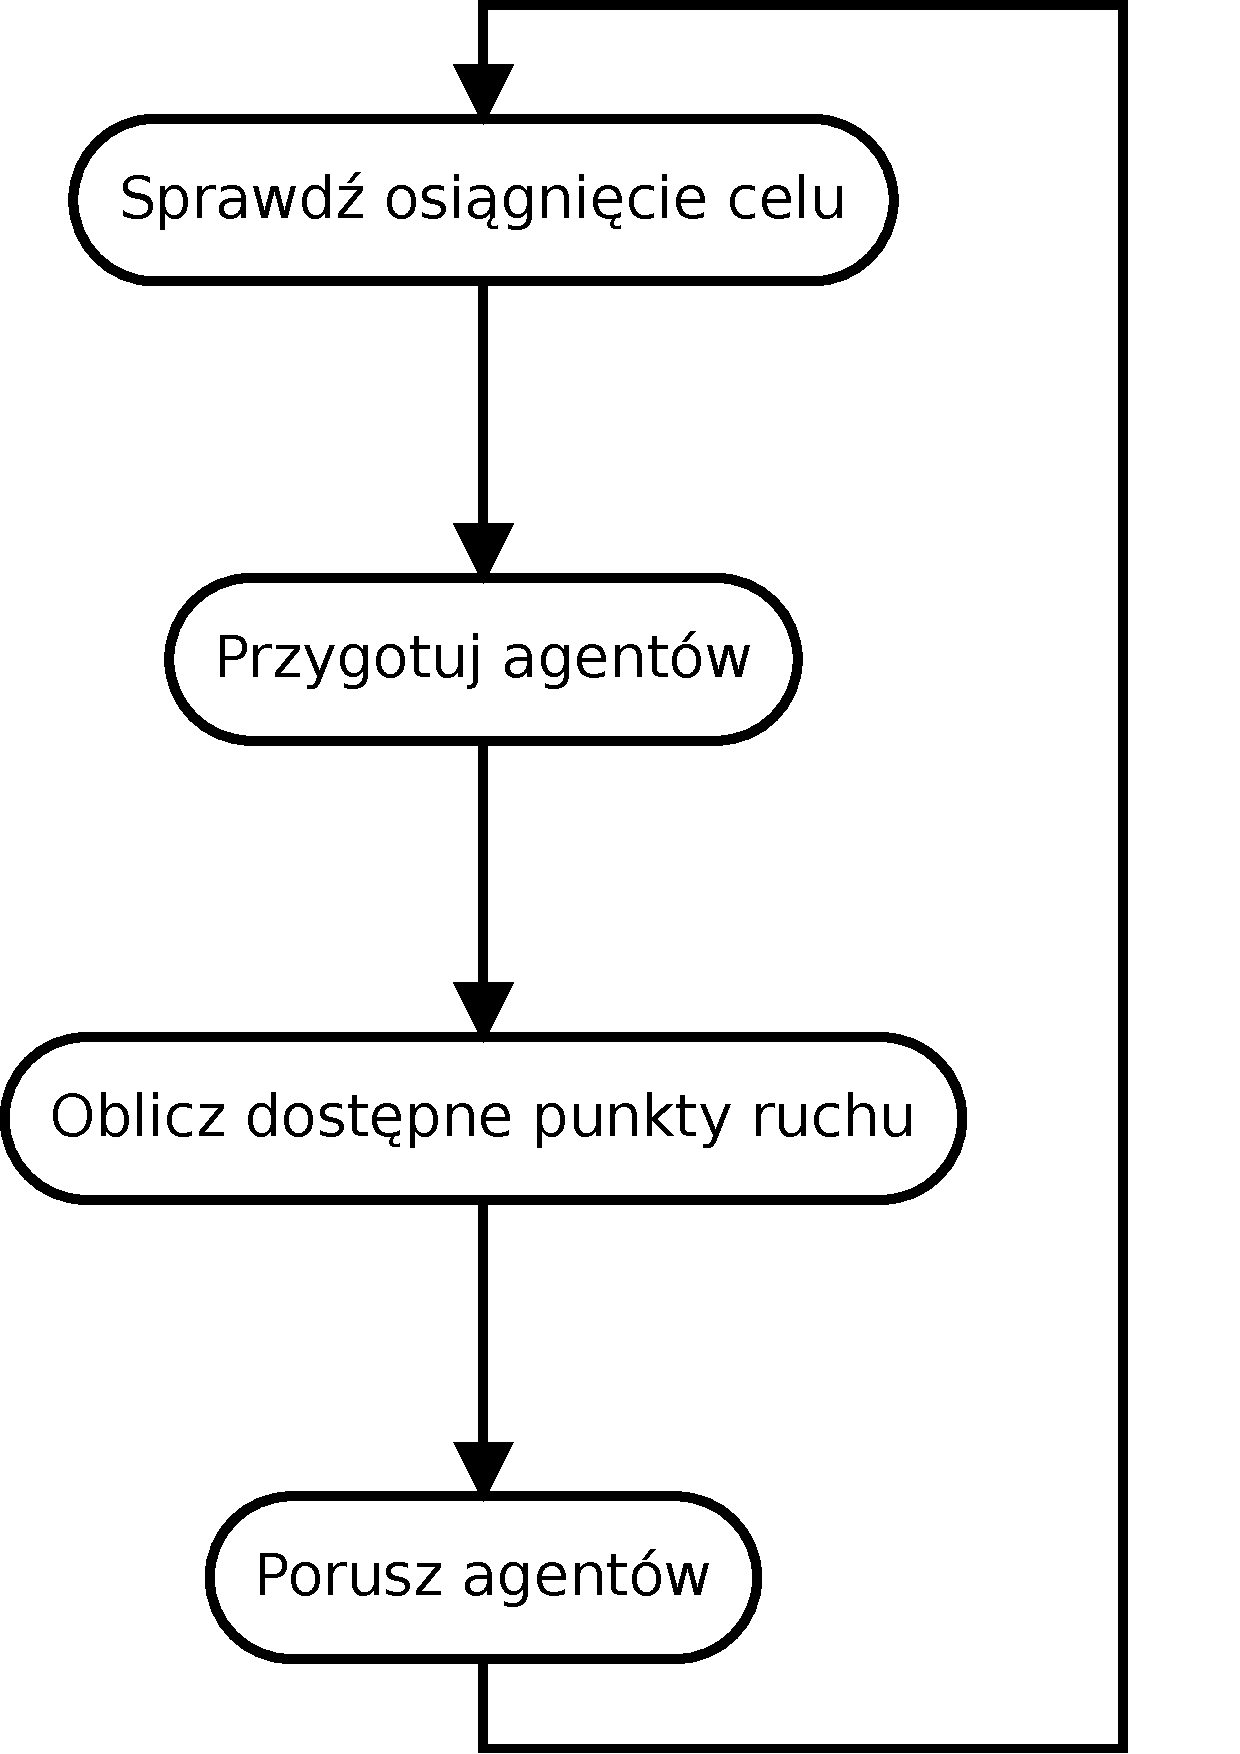
\includegraphics[scale=0.3]{./img/OperationalLoop.pdf}
        \caption{P�tla fazy operacyjnej}
        \label{fig:operloop}
    \end{figure}

\indent Sprawdzanie osi�gni�cia celu s�u�y wyznaczeniu kolejnego celu, o ile poprzedni zosta� osi�gni�ty. Cel mo�na osi�gn�� na dwa sposoby: wchodz�c bezpo�rednio na p�ytk� o zadanych wsp�rz�dnych b�d� wchodz�c na p�ytk� w s�siedztwie celu (w tym przypadku prawdopodobie�stwo uznania celu za osi�gni�ty zale�y od odleg�o�ci p�ytki od niego). Po wyznaczeniu nowego celu aktualizowane s� parametry wykorzystywane przez algorytmy ruchu, jak pocz�tkowa (teoretyczna) minimalna odleg�o�� od celu. \newline
\indent Przygotowanie agent�w polega na wywo�aniu dla ka�dego z nich metody \emph{prepare()} algorytmu przypisanego do p�ytki, na kt�rej agent aktualnie si� znajduje. \newline
\indent Obliczanie dost�pnych w danym obiegu fazy iteracyjnej punkt�w ruchu to przepisanie aktualnej pr�dko�ci maksymalnej ka�dego z agent�w. \newline
\indent W etapie poruszania agent�w agenci rozpatrywani s� cyklicznie. W jednej iteracji (``kroku'') ka�dy z agent�w mo�e wykona� tylko jedn� akcj�,  np. czka� b�d� przemie�ci� si� o jedno (!) pole. Dzi�ki takiemu rozwi�zaniu �aden z agent�w nie jest faworyzowany przy dost�pie do p�l.

\begin{algorithm}
\caption{Faza operacyjna}
\label{alg2}
\begin{algorithmic}
\Procedure{operation\_phase}{}
    \ForAll{agent w galerii}
    \Comment{sprawd� osi�gni�cie celu}
        \If{agent osi�gn�� cel OR agent uzna�, �e osi�gn�� cel}
            \State pobierz kolejny cel z listy
            \State zapisz statystyki dotycz�ce dalszej drogi
        \EndIf
    \EndFor
    \newline
    \ForAll{agent w galerii}
    \Comment{przygotuj agent�w}
        \State \textbf{call} Algorithm.prepare with agent
    \EndFor
    \newline
    \ForAll{agent w galerii}
    \Comment{oblicz punkty ruchu}
        \State punkty\_ruchu\_agenta $\gets$ predkosc\_agenta
    \EndFor
    \newline
    \For{krok od 1 do $v_{max}$}
    \Comment{porusz agent�w}
        \ForAll{agent w galerii}
            \If{agent jest wstrzymywany}
                \State zmniejsz pozosta�y czas wstrzymania
            \ElsIf{agent nie wykorzysta� jeszcze w tym kroku punkt�w ruchu}
                \State \textbf{call} Algorithm.nextIterationStep with agent
                \State \textbf{call} Feature.performAction with agent
                \State wykorzystaj punkt ruchu
            \EndIf
        \EndFor
    \EndFor
\EndProcedure
\end{algorithmic}
\end{algorithm}

Metoda \emph{performAction()}, wywo�ywana dla element�w galerii, ustawia parametry agenta zwi�zane z symulacj� takich zdarze�, jak np. oczekiwanie w kolejce. \newline

Wszystkie algorytmy ruchu implementuj� interfejs \emph{MovementAlgorithm}. Interfejs ten zawiera dwie metody wywo�ywane w fazie operacyjnej dla ka�dego agenta:
\begin{itemize}
\item \emph{prepare()} - wywo�ywana jeden raz, na pocz�tku; s�u�y ustawieniu agenta na odpowiedniej pozycji pocz�tkowej
\item \emph{nextIterationStep()} - wywo�ywana tyle razy, ile agent posiada punkt�w ruchu; obs�uguje ruch "do przodu"; przy ka�dym jej wywo�aniu agent przesuwa si� co najwy�ej o jedno pole (w s�siedztwie Moore'a)
\end{itemize}

    \begin{figure}[H]
        \centering
        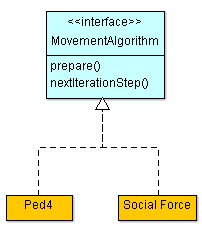
\includegraphics[scale=0.75]{./img/move_algos.png}
        \caption{Interfejs \emph{MovementAlgorithm} i jego realizacje}
        \label{fig:movealgo}
    \end{figure}

        \subsection{Social Force}
        \label{sec:social-force-impl}

Poni�ej przedstawiono pseudokody metody odpowiedzialnej za ruch "do przodu" w algorytmie Social Force:

\begin{algorithm}
\caption{Ruch agenta w algorytmie Social Force}
\label{alg1}
\begin{algorithmic}
\Procedure{nextIterationStep}{}
    \If{brak mo�liwo�ci ruchu}
        \State obr�� agenta
        \Comment{umo�liwia przeszukanie nowych obszar�w}
    \Else
        \State cel $\gets$ wyznacz\_pole\_o\_najwiekszym\_potencjale()
        \State przesu� agenta na docelow� p�ytk�
        \State odzwierciedl kierunek wykonanego ruchu poprzez zmian� zwrotu agenta
    \EndIf
\EndProcedure
\newline
\Function{wyznacz\_pole\_o\_najwiekszym\_potencjale}{}
    \State dostepne\_pola $\gets$ wyznacz\_dostepne\_pola()
    \ForAll{dost�pne pole}
        \State uwzgl�dnij warto�� pola potencja�u innych ludzi i odleg�o�� od celu
    \EndFor
    \If{agent jest zm�czony}
        \State zwi�ksz dodatkowo potencja� dost�pnego pola najbli�ej celu
    \EndIf
    \State pozostaw pola o najwy�szym potencjale \\
    \Return{pole le��ce najbli�ej celu}
\EndFunction
\newline
\Function{wyznacz\_dostepne\_pola}{}
    \State pola\_agenta $\gets$ pola w s�siedztwie von Neumanna le��ce w p�kolu wyznaczonym przez kierunek ruchu agenta
    \State pola\_celu $\gets$ pola w s�siedztwie von Neumanna le��ce w p�kolu wyznaczonym przez kierunek do celu \\
    \Return{pola\_agenta AND pola\_celu}
    \Comment{cz�� wsp�lna zbior�w}
\EndFunction
\end{algorithmic}
\end{algorithm}

\indent Funkcja wyznaczaj�ca dost�pne pola ogranicza mo�liwo� ruchu tak, aby agent albo dalej przemieszcza� si� po dotychczasowej trajektorii, albo skr�ci� w stron� celu. \\
\indent Potencja� pola obliczany jest na podstawie si�y oddzia�ywania innych ludzi (ujemna sk�adowa) oraz odleg�o�ci pola od celu (dodatnia sk�adowa). W przypadku, gdy agent ju� do�� d�ugo zmierza do celu (tzn. przebyta przez niego droga znacz�co przekracza minimaln� drog� konieczn� do osi�gni�cia celu), lecz nie mo�e go osi�gn��, przestaje zwraca� tak� uwag� na innych agent�w – efekt ten zosta� osi�gni�ty przez dodatkowe zwi�kszenie potencja�u dost�pnej p�ytki le��cej najbli�ej celu. \\
\indent W przypadku, gdy brak jest dost�pnych p�ytek, agent obraca si� odrobin� w miejscu, by w nast�pnym kroku zyska� nowe mo�liwo�ci ruchu (ze wzgl�du na zmian� zbioru dost�pnych p�ytek).

\newpage
        \subsection{Wizualizacja i pozyskiwanie danych}
        \label{sec:vis-and-data}

        Wizualizacj� przebiegu symulacji wykonano w oparciu o bibliotek� \textbf{Java Swing} z racji na prostot� implementacji i zadowalaj�ce efekty wizualne, jakie ona dostarcza. Na rysunku \ref{fig:mall-sim-win} zaprezentowano wygl�d g��wnego okna programu podczas przyk�adowej symulacji.

        \begin{figure}[H]
            \centering
            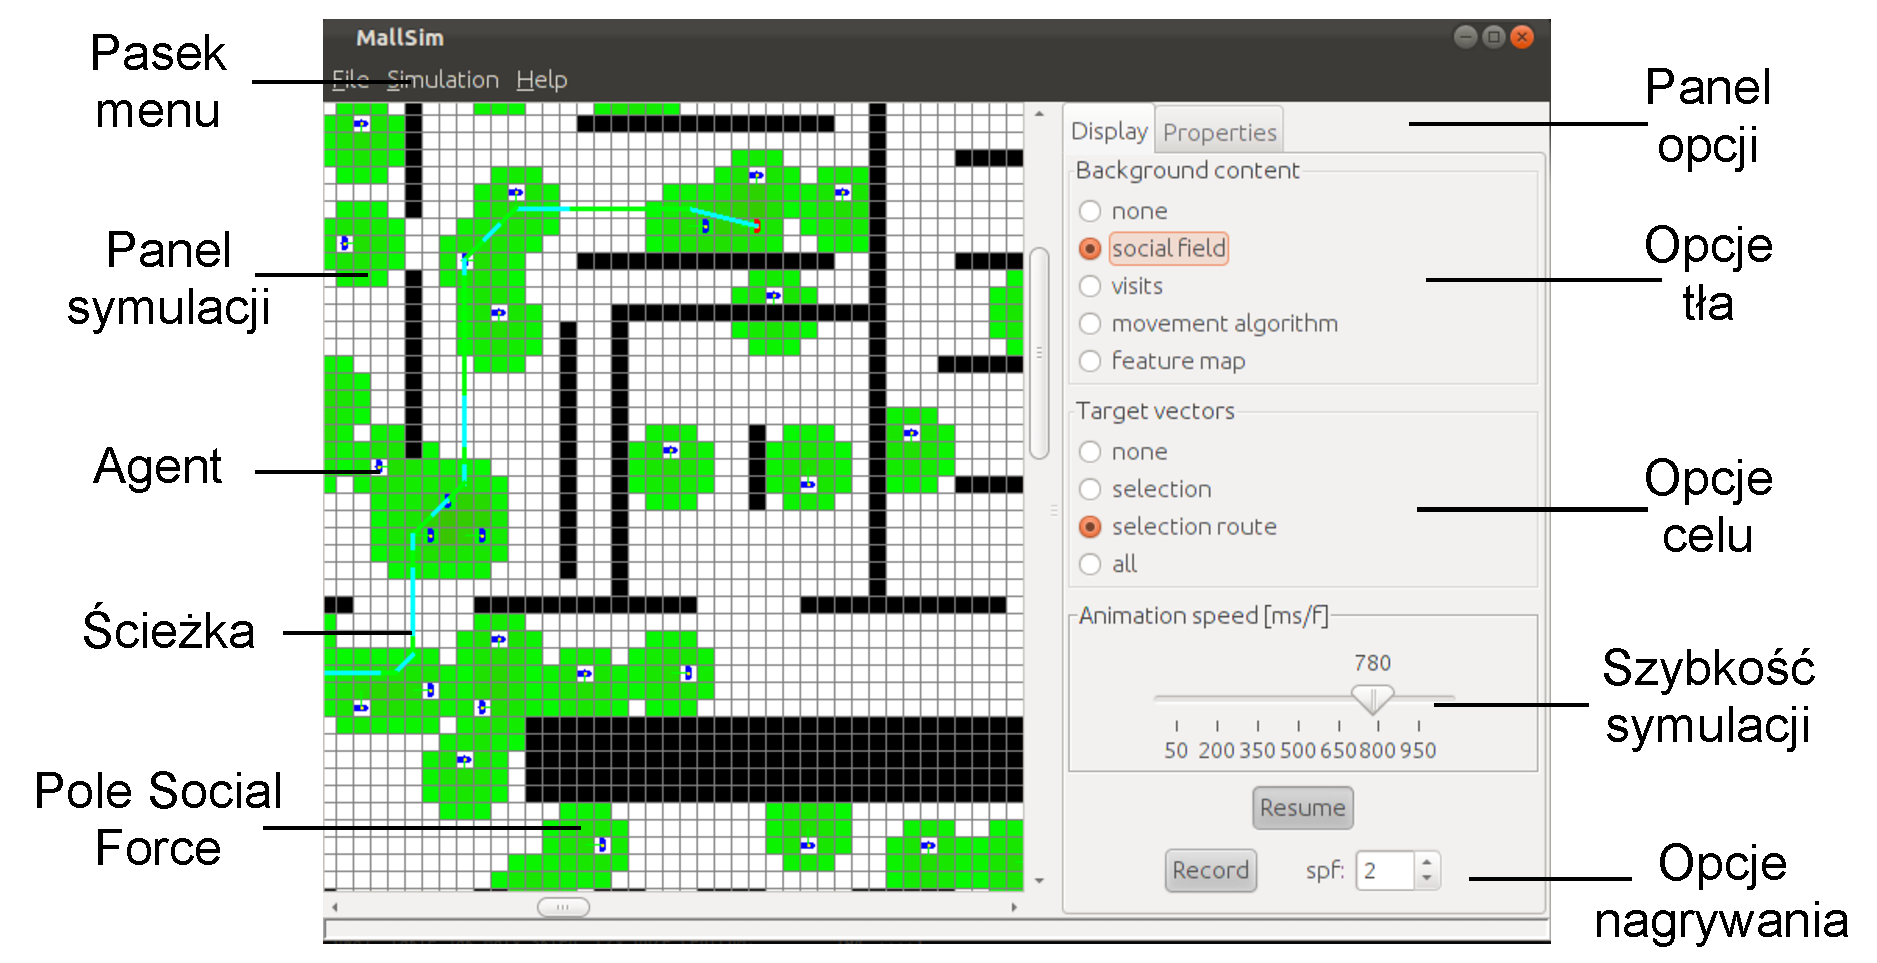
\includegraphics[scale=0.5]{./img/MallSim.pdf}
            \caption{G��wne okno programu.}
            \label{fig:mall-sim-win}
        \end{figure}

        Program udost�pnia wiele konfigurowalnych opcji odpowiadaj�cych za dzia�anie symulacji i jej wizualizacji dost�pnych za po�rednictwem \emph{panelu opcji}:

        \begin{itemize}
            \item \textbf{Opcje t�a} - wyb�r danych wizualizowanych w tle symulacji; do wyboru jedna warto�� z: \emph{brak}, \emph{gradient Social Force}, \emph{rozk�ad odwiedzin danych kom�rek centrum handlowego}, \emph{rozk�ad algorytm�w ruchu}, \emph{rozk�ad stref specjalnych centrum handlowego}.
            \item \textbf{Opcje celu} - opcje wizualizacji celu podr�y agent�w; do wyboru jedna warto�� z: \emph{brak}, \emph{wektor najbli�szego celu wybranego agenta}, \emph{aktualna �cie�ka wybranego agenta}, \emph{wektory najbli�szego celu wszystkich agent�w}.
            \item \textbf{Szybko�� symulacji} - pasek wyboru szybko�ci symulacji (ilo�� milisekund na krok symulacji); warto�ci z przedzia�u 50 do 1000 milisekund.
            \item \textbf{Opcje nagrywania} - opcje odpowiadaj�ce za nagrywanie przepiegu symulacji; obecnie dost�pna jest tylko konfiguracja ilo�ci krok�w na klatk� filmu (\emph{spf}).
        \end{itemize}

        \noindent
        ...oraz \emph{paska menu}:

        \begin{itemize}
            \item \textbf{Seed} - opcje odpowiadaj�ce za \emph{ziarno} symulacji umo�liwiaj�ce kontrolowanie powtarzalno�ci wynik�w.
        \end{itemize}

        W celu u�atwienia pozyskiwania danych do p�niejszej analizy program udost�pnia zak�adk� \emph{Properties} generuj�c� dynamicznie podgl�d parametr�w wybranego agenta oraz mo�liwo�� nagrania przebiegu symulacji za pomoc� biblioteki \textbf{Monte Media Library} - przebieg symulacji zapisywany jest w g��wym katalogu programu w formacie \emph{.avi}.

%\newpage
    \section{Symulacja i analiza wynik�w}
    \label{sec:sim}

    W celu przetestowania poprawno�ci modelu i dzia�ania programu zdecydowano si� przeprowadzi� symulacj� lokalnego centrum handlowego - \href{http://www.galeria-krakowska.pl/}{\emph{Galerii Krakowskiej}}. Przygotowano mapy parteru centrum zaprezentowane na poni�szej ilustracji:

    \begin{figure}[H]
      \centering
      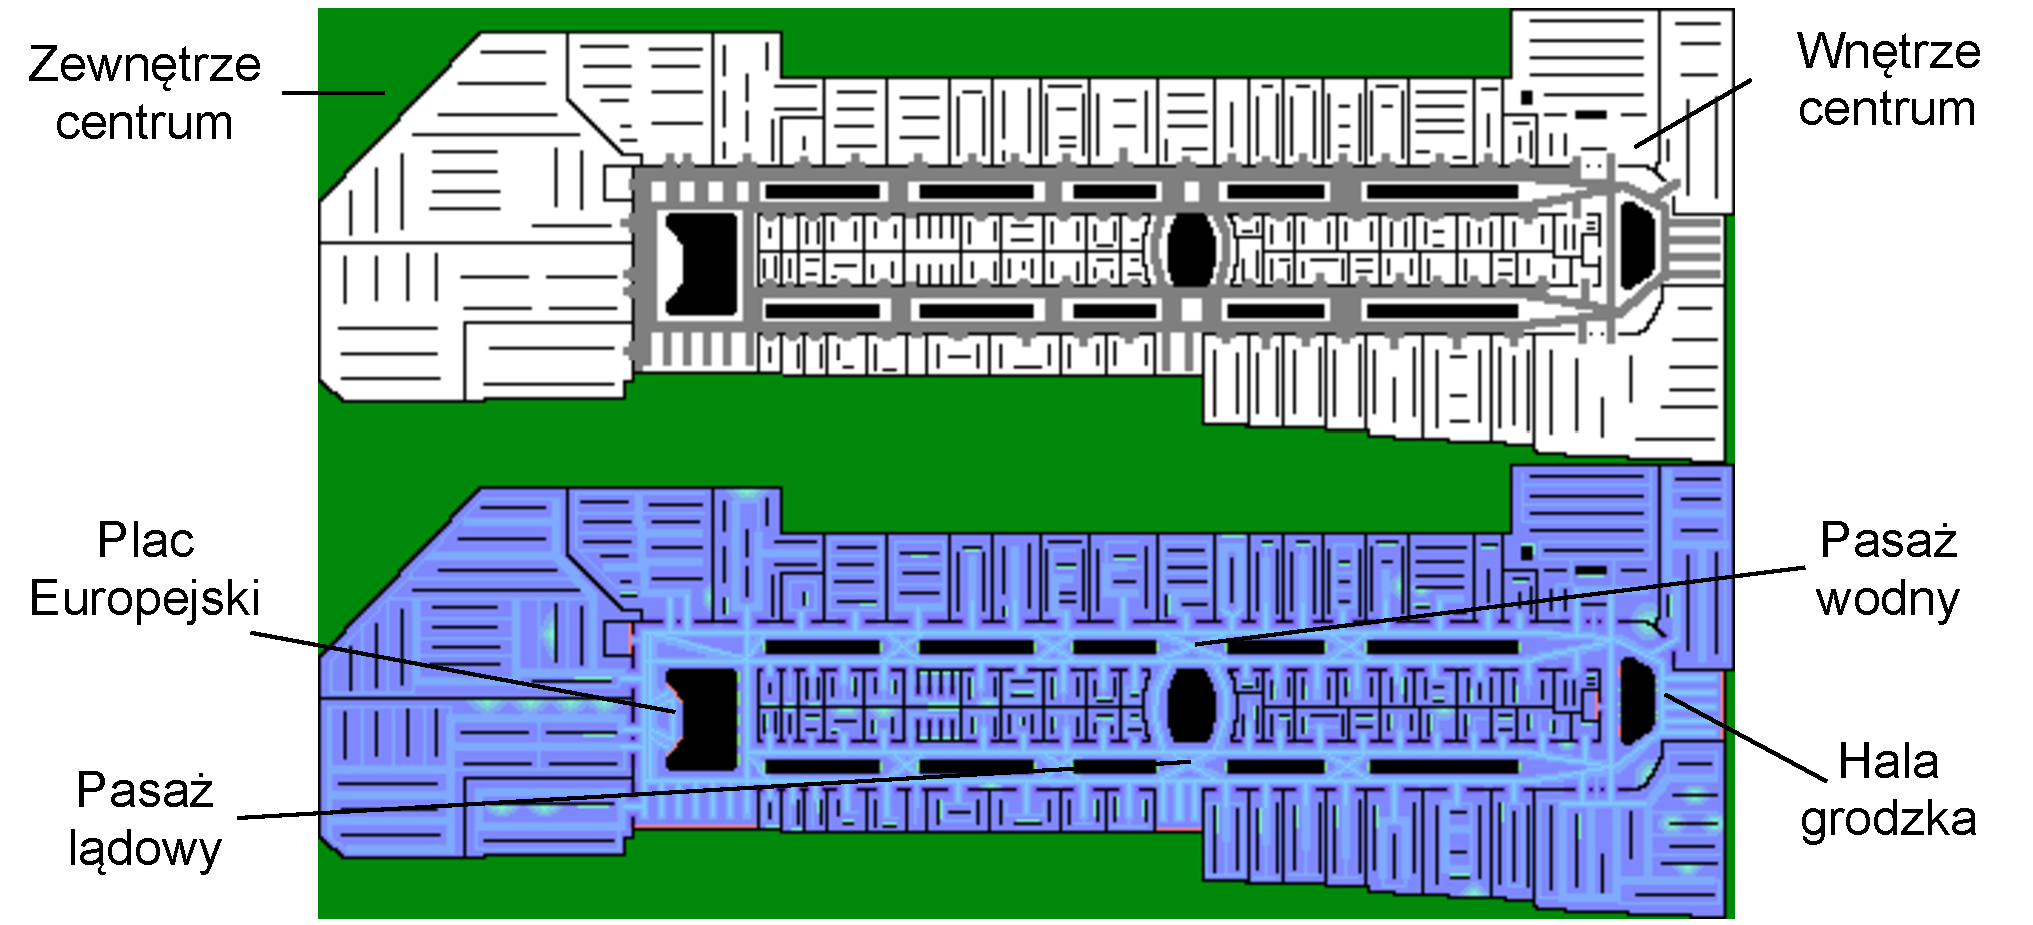
\includegraphics[scale=0.5]{./img/GaleriaKrakowska.pdf}
      \caption{Mapy parteru popularnej \emph{Galerii Krakowskiej}.}
      \label{fig:gk-maps}
    \end{figure}

    \noindent
    Ze wzgl�du na brak dost�pu do danych i dynamiczne zmiany faktycznych rozk�ad�w sklepowych p�ek i alejek mapy parteru symulowanego centrum handlowego, przedstawione na rysunku \ref{fig:gk-maps}, zawieraj� przyk�adowe, proste uk�ady p�ek sklepowych - wizj� autor�w projektu. \\

        \subsection{Kalibracja i walidacja parametr�w symulacji}
        \label{sec:calibration}

        W celu kalibracji i walidacji parametr�w modelu pos�u�ono si� obserwacjami przeprowadzonymi w symulowanym centrum handlowym w wolnym czasie. W zwi�zku z faktem, i� model zastosowany w tej pracy niewiele parametr�w wymagaj�cych kalibracji, z kt�rych wi�kszo�� jest trudna, b�d� niemo�liwa do oszacowania bez du�ej porcji danych statystycznych kalibracj� przeprowadzono w du�ej mierze ``metod� pr�b i b��d�w'' w oparciu o dane zebrane z obserwacji. Uda�o si� w ten spos�b zidentyfikowa� trzy typy agent�w odwiedzaj�cych centrum handlowe (dynamiczny, przeci�tny i ``pensjonariusz''), kt�re r�ni� si� maksymaln� pr�dko�ci� poruszania, ch�ci� do omijania innych agent�w, czy wytrwa�o�ci� w robieniu zakup�w. \\

        Po skalibrowaniu parametr�w dotycz�cych zachowania agent�w przyst�piono do kalibracji parametr�w centrum handlowego, wyra�onych w wi�kszo�ci przez \hyperref[fig:mall-features]{map� rozk�adu stref specjalnych} centrum handlowego, kt�ra jest wykorzystywana przez algorytm wyszukiwania �cie�ek. Kalibracja przebiega�a ze wzgl�du na dwa kluczowe aspekty symulacji - czas generowania �cie�ek oraz zachodzenie abstrakcyjnych zjawisk opisanych w nast�pnej sekcji. Kalibracj� ponownie przeprowadzono w oparciu o dane pochodz�ce z w�asnych obserwacji i ``zrdrowego rozs�dku'', niestety administracja \emph{Galerii Krakowskiej} nie udzieli�a autorom pracy dost�pu do istotnych danych, kt�re umo�liwi�yby stworzenie lepszej mapy rozk�adu stref specjalnych, kt�ra dok�adniej oddawa�aby rzeczywisty charakter \emph{Galerii Krakowskiej}. \\

        Walidacj� opracowanych parametr�w przeprowadzono konfrontuj�c wyniki symulacji z rzeczywistymi do�wiadczeniami wyniesionymi z symulowanego centrum handlowego. Por�wnanie wynik�w symulacji do poczynionych obserwacji rzeczywistego zachowania ludzi zawarto w nast�pnych sekcjach.

        \subsection{Uzyskane wyniki ilo�ciowe i jako�ciowe}
        \label{sec:results}

        Uzyskane wyniki spe�niaj� wszystkie za�o�enia postawione w sekcjach \ref{sec:mall-model} i \ref{sec:move-model} i s� bardzo zbli�one do rzeczywistych zachowa� ludzi w centrum handlowym. Agenci poruszaj� si� zgodnie z wytyczonymi �cie�kami, kt�re dobierane s� w taki spos�b, by dany agent odwiedzi� wiele sklep�w w centrum handlowym:

        \begin{figure}[H]
          \centering
          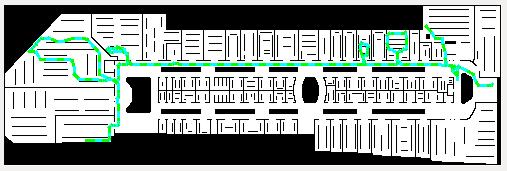
\includegraphics[scale=0.7]{./img/route.png}
          \caption{Wybrana przez algorytm �cie�ka prowadz�ca agenta po centrum handlowym.}
          \label{fig:res-route}
        \end{figure}

\noindent
Modeluje to strategiczne plany ludzi, kt�rzy odwiedzaj�c centrum handlowe przewa�nie planuj� sp�dzi� tam wi�cej czasu. Opisany w sekcji \ref{sec:path-finding} algorytm wyboru �cie�ek prowadzi do powstania realistycznego routingu ludzi w centrum handlowym:

        \begin{figure}[H]
          \centering
          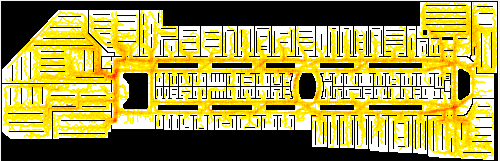
\includegraphics[scale=0.7]{./img/routing.png}
          \caption{Realistyczny routing agent�w w centrum handlowym.}
          \label{fig:res-routing}
        \end{figure}

\noindent
Spontanicznie tworz� si� pasy ruchu, kt�rymi ludzie pod��aj� do celu swojej podr�y:

        \begin{figure}[H]
          \centering
          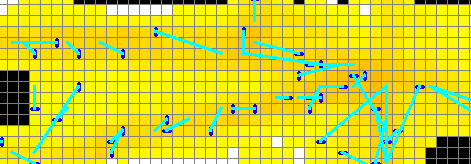
\includegraphics[scale=0.7]{./img/lanes.png}
          \caption{Samoistne tworzenie si� pas�w ruchu.}
          \label{fig:res-lanes}
        \end{figure}

\noindent
Zupe�nie jak w prawdziwym centrum handlowym, agenci preferuj� poruszanie si� �rodkiem korytarza w miar� mo�liwo�ci, o czym �wiadczy wi�ksza warto�� ``temperatury'' na �rodku poni�szej ilustracji:

        \begin{figure}[H]
          \centering
          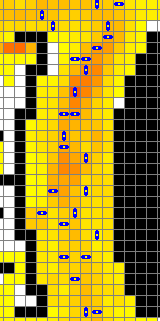
\includegraphics[scale=0.7]{./img/middle.png}
          \caption{Agenci preferuj�cy �rodek korytarza.}
          \label{fig:res-middle}
        \end{figure}

\noindent
Takie zachowanie prowadzi do tworzenia si� skupisk ludzi (\emph{ang. flocking}), co wp�ywa na preferencje odleg�o�ciowe zaanga�owanych agent�w i zmian� ich gradient�w \emph{Social Force}. Zmiana ta poci�ga za sob� roz�adowanie zatoru - model osi�ga stabilno�� automatycznie si� reguluj�c:

        \begin{figure}[H]
          \centering
          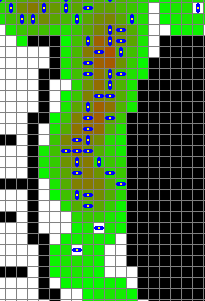
\includegraphics[scale=0.7]{./img/bottleneck.png}
          \caption{Samoistne tworzenie si� zgrupowa� ludzi - \emph{flocking}.}
          \label{fig:res-bottleneck}
        \end{figure}

R�wnie interesuj�ce jest powstawanie abstrakcyjnych zachowa� wymienionych w sekcji \ref{sec:mall-model}. Algorytm \hyperref[sec:tactical]{fazy taktycznej} uwzgl�dnia \emph{atrakcj�} agent�w do r�nych, interesuj�cych stref centrum handlowego, co zaprezentowano na rysunku \ref{fig:res-attraction}.

        \begin{figure}[H]
          \centering
          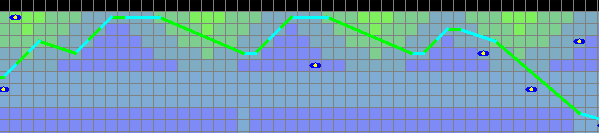
\includegraphics[scale=0.7]{./img/attraction.png}
          \caption{Uwzgl�dnianie miejsc przyci�gaj�cych uwag� w �cie�ce agenta.}
          \label{fig:res-attraction}
        \end{figure}

\noindent
Obserwowa� mo�na naturalne zachowania, takie jak zatrzymanie si� przed oknem wystawowym, cz�sto obserwowane w prawdziwych centrach handlowych:

        \begin{figure}[H]
          \centering
          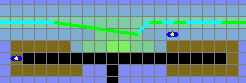
\includegraphics[scale=0.7]{./img/attraction2.png}
          \caption{Charakterystyczne zboczenie z trasy celem osi�gni�cia atraktora.}
          \label{fig:res-attraction-2}
        \end{figure}

\noindent
Agenci bardzo ch�tnie grupuj� si� by obserwowa� r�ne ciekawe zjawiska obecne w symulowanym centrum handlowym - wszystko dzi�ki umieszczonym tam \hyperref[sec:attractors]{atraktorom}:

        \begin{figure}[H]
          \centering
          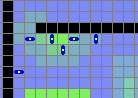
\includegraphics[scale=0.7]{./img/attraction3.png}
          \caption{Agenci w obr�bie atraktora.}
          \label{fig:res-attraction-3}
        \end{figure}

\hyperref[sec:queues]{Kolejki}, podobnie jak atraktory, brane s� pod uwag� ju� w fazie taktycznej dzia�ania algorytmu - agenci dokonuj�cy zakupu podchodz� do kasy i oczekuj� na obs�ug� imituj�c zachowanie prawdziwych ludzi:

        \begin{figure}[H]
          \centering
          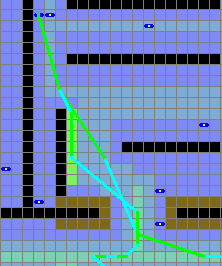
\includegraphics[scale=0.7]{./img/queueing.png}
          \caption{Uwzgl�dnianie sklepowych kas i kolejek w �cie�ce agenta.}
          \label{fig:res-queueing}
        \end{figure}

\noindent
Zachowanie to uda�o si� osi�gn�� pomimo dzia�ania algorytmu \hyperref[sec:operational]{Social Force}, kt�ry nakazuje agentom trzymanie dystansu do siebie nawzajem:

        \begin{figure}[H]
          \centering
          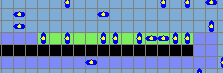
\includegraphics[scale=0.7]{./img/queueing2.png}
          \caption{Agenci oczekuj�cy na swoj� kolej.}
          \label{fig:res-queueing-2}
        \end{figure}

W podobny spos�b osi�gni�to \hyperref[sec:holders]{wstrzymanie agent�w} - symuluj�ce wszelkiego rodzaju odpoczynki i czasy oczekiwania zdarzaj�ce si� w centrum handlowym:

        \begin{figure}[H]
          \centering
          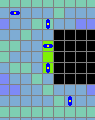
\includegraphics[scale=0.7]{./img/hold.png}
          \caption{Agenci odpoczywaj�cy na �awce (w obr�bie op�niacza).}
          \label{fig:res-hold}
        \end{figure}

Interesuj�cym jest fakt, i� nawet pomimo zastosowania skomplikowanych algorytm�w routingu i wyszukiwania �cie�ek uda�o si� otrzyma� niemal stu procentowe pokrycie centrum handlowego. Agenci bezproblemowo osi�gaj� wszystkie jego pomieszczenia, co doskonale oddaje charakterystyki prawdziwego centrum handlowego i zachowanie ludzi tam obecnych.

        \begin{figure}[H]
          \centering
          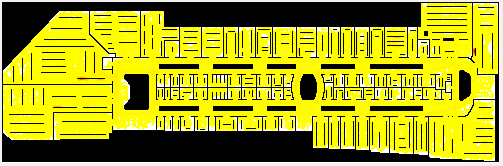
\includegraphics[scale=0.7]{./img/coverage.png}
          \caption{Pokrycie centrum handlowego.}
          \label{fig:res-coverage}
        \end{figure}


Dodatkowo do dokumentacji projektu za��czono kilka film�w pokazuj�cych dzia�anie symulacji i powstawanie wy�ej opisanych zachowa�:

        \begin{itemize}
          \item \textbf{overview.avi} - Prezentacja r�nych aspekt�w wizualizacji symulacji: zbli�anie, oddalanie, przesuwanie planu galerii, rozk�ad pola potencja�u, mapa ``temperatury'' (licznik odwiedzin p�l).

          \item \textbf{movement.avi} - Przyk�ad formowania si� ``pas�w ruchu'' na prostych odcinkach korytarza (g�rna cz�� animacji) dzi�ki u�yciu algorytmu Ped-4. Problemy ze wsp�istnieniem obok siebie algorytm�w Ped-4 i Social Force (patrz: ruch agent�w po wygi�tych w �uch korytarzach) - piesi zawracaj� b�d� ``kr�c� si� w k�ko'' powoduj�c zator.

          \item \textbf{queue\_attractor.avi} - Dzia�anie kolejek (po prawej stronie) oraz atraktor�w (w �rodku i po lewej stronie) - agenci ch�tnie zbli�aj� do takich stref. Wej�cie na atraktor albo kolejk� powoduje wstrzymanie agenta na okre�lony czas.

          \item \textbf{social\_force.avi} - Przyk�ad omijania innych klient�w z uwzgl�dnieniem stref komfortu dzi�ki zastosowaniu algorytmu Social Force.

          \item \textbf{visits.avi} - Animacja pokazuj�ca przep�w ludzi w galerii handlowej. Wyra�nie wida� du�y, skoncentrowany ruch po korytarzach oraz niewielki i rozproszony ruch po obszarach sklep�w.

          \item \textbf{wall\_error.avi} - Przyk�ad b��d�w wyznaczania �cie�ki skutkuj�cy niemo�liwo�ci� osi�gni�cia wyznaczonego celu z powodu natrafienia na �cian�. Przyczyn� jest przedwczesne uznanie wcze�niejszego celu (le��cego w tym przypadku na szczycie �ciany) za osi�gni�ty oraz wyznaczenie kolejnego celu w miejscu niewidocznym z pozycji agenta w chwili uznania poprzednieg celu za osi�gni�ty.
        \end{itemize}

        \subsection{Wyniki symulacji a rzeczywisto��}
        \label{sec:sim-vs-reality}
Wyniki symulacji do�� dobrze oddaj� charakter zjawisk obserwowanych w rzeczywistej galerii handlowej.

W korytarzach obserwujemy formowanie si� ``pas�w ruchu'' - ludzie staraj� si� i�� jeden za drugim w kolumnie, pr�buj� wyprzedza� si� tylko wtedy, gdy nie nadchodzi nikt z naprzeciwka. We wn�trzach sklep�w dzieje si� na odwr�t - brak po�piechu sprawia, �e klienci wi�ksz� wag� przywi�zuj� do nie naruszania swoich stref komfortu.

Na podgl�dzie odwiedzonych p�ytek widzimy, �e klienci preferuj� ruch �rodkiem korytarzy, jednak gdy zajdzie taka konieczno�� korzystaj� z ca�ej jego dost�pnej szeroko�ci.

W przypadku sklep�w rozk�ad odwiedzanych miejsc jest znacznie bardziej r�wnomierny, czego r�wnie� mo�na by�o oczekiwa� - wewn�trz sklepu (o ile nie jest to dyskont spo�ywczy) klient porozgl�da si� i zapoznaje z ofert� sklepu, a uwag� r�nych os�b przyci�gaj� r�ne produkty. Warto r�wnie� zauwa�y�, �e w przypadku niewielkich sklep�w (typu: 101 drobiazg�w, Świat Kawy i Herbaty) stosunkowo niewielu klient�w wchodzi g��biej do �rodka - wi�kszo�� po wej�ciu rozgl�da si� chwil� i wychodzi. Zachowanie takie jest cz�sto obserwowane w galeriach handlowych.

Analiza wynik�w symulacji wykaza�a r�wnie� konieczno�� dalszej kalibracji (oraz ewentualnie cz�ciowej zmiany metodologii) procesu wyznaczania �cie�ek. Na chwil� obecn� nie uda�o si� w pe�ni wyeliminowa� niekorzystnego zjawiska ``forsowania �ciany'' przez agent�w spowodowanego r�wnoczesnym wyst�pieniem dw�ch zdarze�: przedwczesnym uznaniem celu za osi�gni�ty oraz wyznaczeniu kolejnego celu w miejscu niewidocznym z aktualnej pozycji agenta. Przyk�ad takiej sytuacji pokazano poni�ej: je�li agent uzna punkt $A$ za osi�gni�ty jeszcze przed omini�ciem �ciany, wektor celu prow�dz�cy do punktu $B$ spowoduje ruch agenta wzd�� �ciany i pr�b� jej p�niejszego ``sforsowania''.

\begin{figure}[H]
  \centering
  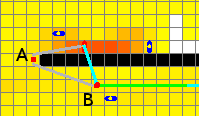
\includegraphics[scale=0.7]{./img/wallsmasher.png}
  \caption{Forsowanie �ciany przez wybranego agenta.}
  \label{fig:bug-wallsmasher}
\end{figure}




% itd.
% \appendix
% \include{dodatekA}
% \include{dodatekB}
% itd.

\bibliography{bib}
\bibliographystyle{alpha}

% Kolejne pozycje bibliograficzne:
% *) algorytm A*

\end{document}
